\chapter{CountNet}

\section{Introduction}%
\label{sec:introduction}

\begin{figure}[t]
  \centering
  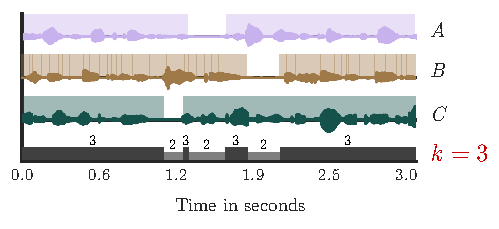
\includegraphics[width=0.8\columnwidth]{Chapters/08_Analysis_CountNet/figures/teaser.pdf}
  \caption{Illustration of our application scenario of three concurrent speakers (A, B, C) and their respective speech activity. Bottom plot shows the mixture (input), the number of concurrently active speakers and its maximum \(k\) which is our targeted output.}%
  \label{fig:teaser}%
\end{figure}

% Introduce the task of estimating the maximum number of concurrent speakers in a single-channel mixture.
% * Lets start right into the task
% Source Separation (count estimate make blind SS fully blind)
In a ``cocktail-party'' scenario, one or more microphones capture the signal from many concurrent speakers. In this setting, different applications may be envisioned such as localization, crowd monitoring, surveillance, speech recognition, speaker separation, etc.
When devising a system for such a task, it is typically assumed that the actual number of concurrent speakers is known.
This assumption turns out to be of paramount importance for the effectiveness of subsequent processing.
Notably, for separation algorithms~\cite{common10},
real-world systems do not straightforwardly provide information about the actual number of concurrent speakers.
% Assuming knowledge of speaker counts thus appears more as convenient than as realistic in practice.
It, therefore, is desirable to close the gap between theory and practice by devising reliable methods to estimate the number of sound sources in realistic environments.
Surprisingly, very few methods exist for this purpose in an audio context, in particular from a single microphone recording.

\par

% TODO: Maybe mention model selection, spectral clustering, gap statistics etc.
%% Transition paragraphs
% Describe two ways of getting the number of speakers: Counting vs Estimation
From a theoretical perspective, estimating the number of concurrent speakers is closely related to the more difficult problem of \textit{identifying} them, which is the topic of speaker diarization~\cite{angueramiro12, rouvier13, rouvier15, ramaiah17}.
Intuitively, if a system is able to tell who speaks when, it is naturally also able to tell how many speakers are actually active in a mixture.
We call this strategy ``counting by detection''.
A good working diarization system would be able to sufficiently address the speaker count estimation problem using this strategy.
However, it appears to be a very complex problem to tackle when one is only interested in the number of concurrent speakers.
Furthermore, as diarization only works when a clear segmentation is possible, the first step of such a strategy often is to find homogeneous segments in the audio where only one speaker is active.
The segment borders can be found by speaker change detection~\cite{Yin17}.
These homogeneous segments are used to discriminate and temporally locate the speakers within a given recording.
When sources are simultaneously active, as in real cocktail party environments, such a segmentation is hardly possible.
In fact, overlapping speech segments typically are a major source of error in speaker diarization~\cite{angueramiro12}.
\par
To improve the robustness of these detection-based methods, a number of approaches attempt to detect and possibly reject the overlapping speech segments to improve performance~\cite{boakye08, huijbregts09}.
Overlap detection has since emerged into its own line of research with many recent publications such as~\cite{geiger13, shokouhi17, hagerer17, andrei17}.
Overlap detection can be seen as a binarized version of the count estimation problem where the number of speakers equals to one (\emph{no overlap}) or more than one (\emph{overlap}).
It is, therefore, possible to apply a count estimation system for the overlap detection problem but not vice versa.
Also, an overlap detection system cannot be easily utilized in a source separation system.
In fact, it should be noted that before the arrival of deep learning based separation systems, models required long context and in such a case, for methods like NMF, the number of concurrent speakers could be introduced as a regularization term~\cite{lefevre11}.
In recent years, however, large improvements were achieved by deep learning based methods~\cite{yu16, hershey16} at shorter segment duration (often 1-5 seconds).
In such approaches, it becomes possible to apply separation only when its ``needed''.
In this scenario, a method of estimating the maximum number of concurrent speakers becomes useful and in some cases essential.
% * Briefly explain differences between counting by detection and directly estimate a count
% with respect to regression or classification. We want to directly estimate the count!
% * Explain how humans count/estimate.
% * Indications that humans are able to do directly estimate vision.
% * How do humans do count and why can't machines?
\par
When speaker overlap is as prevalent as in a ``cocktail-party'' scenario, developing an algorithm to detect the number of speakers is challenging.
This is in contrast to humans whom we know are excellent in segregating one source from a mixture~\cite{bregman} and tend to use this skill to perceptually segregate speakers before they can estimate a count, as highlighted, e.g.\ in~\cite{kawashima15}.
As shown in~\cite{kashino96, kawashima15}, humans are able to correctly estimate up to three simultaneously active speakers without using spatial information.
Similarly, in music, psycho-acoustic researchers came up with a ``one-two-three-many'' hypothesis~\cite{huron89, stoeter13, schoeffler13}.
The question if machines could outperform humans, or if they are subject to similar limitations, remains to be answered.
%
\par
Identifying isolated sources in realistic mixtures is challenging~\cite{bregman} and psychology studies in vision~\cite{jevons1871} have shown that humans can instantly estimate the number of objects without actually counting and therefore identifying them.
This phenomenon is known as \textit{subitizing} and has been inspiring research in vision~\cite{chattopadhyay17}.
Since there are indications that the auditory system is also capable of subitizing sources~\cite{hoopen79}, we transfer this fact to the audio domain and directly attempt in this study to estimate the number of audio sources instead of counting them after identification.
We refer to this strategy as ``direct count estimation''.

\par

%% State-of-the-art
% Reference counting methods with restrictions to audio and concurrent speech.
% * Single-channel vs. multi-channel (harder problem is single-channel)
Directly estimating the number of sources in audio mixtures has many applications and appears as a reasonable objective that mimics the process of human perception.
Since humans do have two ears that provide spatial diversity, a first natural idea to imitate human performance is to exploit \textit{binaural} information to proceed to source count estimation.
In terms of signal processing, this is achieved by estimating directions of arrival (DoA) and clustering them~\cite{loesch08, araki09, arberet10, pavlidi12, drude14_icassp, mirzaei15, walter15, Pasha17_reverb}.
However, many audio devices provide only a single microphone signal, and being able to also count sources, in that case, is desirable. Thus, the single-channel scenario has been considered in many studies.
\par
One of the first methods was proposed in 2003 by Arai~\cite{arai03}.
It is based on the assumption that speech mixed from more than one speaker has a more complex amplitude modulation pattern than a single speaker.
The modulation pattern is aggregated and used as a decision function to distinguish between different numbers of speakers.
In~\cite{sayoud10}, the authors propose an energy feature based on temporally averaged mel filter outputs.
The number of concurrent speakers was determined by manually determining thresholds that best match individual speaker counts.
In a more recent work,
Xu et.al.~\cite{xu13} estimate the number of speakers by applying hierarchical clustering to fixed-length audio segments using mel frequency cepstral coefficients (MFCCs) and additional pitch features.
The method assumes the presence of at least some non-overlapped speech and was evaluated on real-world data of 20 hours duration.
An average count estimation error of one speaker is reported using excerpts of eight-minutes duration and featuring up to eight speakers.
In another vein, Andrei et.al.~\cite{andrei15} proposed an algorithm which correlates single frames of multi-speaker mixtures with a set of single-speaker utterances.
The resulting score was then used to estimate the number of speakers using thresholds.
\par
%% What is the gap?
In all the aforementioned methods, the speaker count estimation problem was devised.
The different strategies undertaken there rely on classical and grounded signal processing strategies and exhibit fair performance in a controlled setup.
However, our experience shows (see Section~\ref{sec:evaluation}) that they leave much room for improvement when applied to more diverse and challenging signals than those corresponding to their targeted applications, notably in the case of many different and constantly overlapping speakers.
% * Existing single-channel methods require segments where only a single speaker is active.
This is due to their main common weakness, which is to rely on the assumption that there are segments where only one speaker is active, in a way that is similar to the classical speaker diarization studies mentioned before.
In~\cite{stoeter17} a first data-driven approach based on a recurrent network was presented, motivated by the recent and impressive successes of deep learning approaches in various audio tasks like speech separation~\cite{yu16, hershey16, grais17} and speaker diarization~\cite{yella14, hruz16, garciaromero17}.
The methods proposed in~\cite{stoeter17} to address speaker count estimation using deep learning were built
upon recent methods to count objects in images, which is a popular application with many contributions
from the deep learning community~\cite{wang15,chattopadhyay17,khan16,segui15,zhang15,arteta16,marsden16,boominathan16,zhang2015salient}.
In~\cite{stoeter17} two main paradigms were evaluated: a) count estimation as regression problem, where the systems are directly trained to output the number of objects as a point estimate, and b) classification, where every possible number of objects is encoded as a different class and the output of a predicting system corresponds to a probability distribution over these classes.
The results of the proposed method indicated that a classification based neural network performed better than one based on regression.
One drawback, however, is that the maximum number of speakers (the number of classes) is known in advance.

Many tasks in machine learning are formulated as classification problems and many models were proposed to address count estimation in this setup~\cite{segui15, zhang2015salient, khan16}, with good performance.

\par

In this study, we build upon~\cite{stoeter17} and focus on the network architecture design, as well as on finding limitations for different test scenarios.
This work makes the following contributions:
%% List of Contributions
% * Defining the problem of Estimating Number of Concurrent Sources.
i) we generalize the problem formulation by fusing classification and regression, which allows estimating discrete outputs while controlling the error term. This is done by picking a point estimate from a full posterior distribution provided by the deep architectures;
% * Influence of three different problem formulations: regression, poisson regression. classification
% * Solution: Investigation of several deep learning architectures.
ii) in addition to the recurrent network introduced in~\cite{stoeter17}, we propose alternative speaker-independent neural network architectures based on the convolution operation to improve count estimation.
Each of the proposed networks is adjusted to estimate the number of speakers from audio segments of 5 seconds;
iii) we test the performance of these networks in multiple experiments and compare them to several baseline methods, pointing out possible limitations.
Furthermore, we present a statistical analysis of the results to determine whether classification outperforms regression for all architectures;
% * Experiments aim to identify the learned strategy.
iv) we conducted a listening experiment to relate the best-performing machine to human performance.
We describe one of the strategies taken by the data-driven approach that might explain its superior performance.
Finally, for the sake of reproducibility, the trained networks (models), as well as the test dataset, are made available on the accompanying website\footnote{\url{https://www.audiolabs-erlangen.de/resources/2017-CountNet}.}.
\par
%% Organisation
The remainder of this paper is organized as follows. In Section~\ref{sec:problem_formulation}, we describe the count estimation problem formally and the general ideas we propose to tackle it.
In Section~\ref{sec:supervised_learning}, we propose several architectures, each of them adjusted to estimate the number of speakers from short audio segments of 5~s.
In Section~\ref{sec:hyperparameters}, we then assess several common hyperparameters for all of our proposed architectures, so that we are able to propose a single, best-performing model.
In Section~\ref{sec:evaluation} this model is compared to several baseline systems under various acoustical conditions.
Additionally, we compare the proposed method to human performance.
We point out possible limitations and provide indications for the strategy being taken by the DNN in Section~\ref{sec:ablation} before we conclude in Section~\ref{sec:conclusion}.

\section{Problem Formulation}%
\label{sec:problem_formulation}
% introduce the section
We consider the task of estimating the maximum number of concurrent speakers \( \cardinality \in \mathbb{Z}^{+}_{0} \) in a single-channel audio mixture \(\mathbf{x}\).
This is achieved by applying a mapping from \(\mathbf{x}\) to \(\cardinality \).
We now provide details on the notations, the general structure of the method, and various ways to exploit the deep learning framework to estimate \(\cardinality \).

\subsection{Signal Model}%
\label{ssec:signal_model}
Let \(\mathbf{x}\) be a time domain vector with \(N\) samples, representing a linear mixture of \(L\) single speaker speech signal vectors \(\mathbf{s}_l\).
The value observed at time instant~\(n\) for the mixture is given by~$x_n$ and for the individual speech segments by~$s_{nl}$.
The mixture then results in
%
\begin{equation}
  x_n = \sum_{l=1}^{L}{s_{nl}} \; \forall n \in \mathbb{Z}^N.
  \label{eq:mixing_model}
\end{equation}
%
Naturally, each speaker~$l=1,\dots,L$ is not active at every time instant.
On the contrary, we assume there is a latent binary \textit{speech activity} variable~$v_{nl}\in \left\{ 0,1 \right\}$ that is either provided by a ground truth annotation or computed using a voice activity detection method.
% \begin{equation}
% v_{nl}=\begin{cases}
% 1 & \text{if }\left|s_{nl}\right|>0\\
% 0 & \text{otherwise}.
% \end{cases}\label{eq:definition_speech_activity}
% \end{equation}

Our objective of estimating the maximum number of concurrent speakers can now be formulated as
%
\begin{equation}
k=\underset{n}{\max}\left(\sum_{l = 1}^{L} v_{nl}\right) \; n \in \{ 1,\ldots, N \}
\label{eq:definition_k}.
\end{equation}
%
As can be seen, our proposed task of estimating $k\leq L$, is more closely related to source separation whereas the estimation of \(L\) is more useful for tasks where speakers do not overlap.
For instance, three non-overlapping speakers would result in \(L = 3\) and \(\cardinality = 1\).
It should be noted that at short time scales both task definitions provide the same outcome because on such a time scale the speaker configuration usually does not change. The problem arises for long-term recordings (e.g. larger than ten seconds) which are not considered in this work.
In any case, we want to emphasize that in all then experiments presented in this paper, we made sure that for all audio segments $L = k$.
\par
In the rest of this work, we assume that no additional prior information about the speakers is given to the system except possibly the maximum number of concurrent speakers~$k_{\max}$, that is application-dependent and represents an upper bound for the estimation.

While speaker diarization would mean estimating the whole speech activity matrix~$v_{nl}$, our problem of estimating only~$k$ in~(\ref{eq:definition_k}) is more abstract as it requires a direct estimation of the count as advocated in Section~\ref{sec:introduction}.

In Figure~\ref{fig:teaser}, we illustrate our setup in a ``cocktail-party'' scenario featuring~$L=3$ unique speakers.
At any given time, we see that at most~$k=L=3$ speakers are active at the same time and~$k=2$ could be the outcome if a smaller excerpt would be evaluated.
By processing such excerpts in a sliding-window fashion, our proposed solution can be applied straightforwardly to context sizes commonly used in source separation.
Furthermore, our proposed system can be used also to detect overlap ($k > 1$), which can be useful as a pre-processing step for diarization.

Now, the system we propose is actually not inputting the signal vector $\mathbf{x}$, but rather a Time-Frequency (TF) representation as the absolute value of the short-term Fourier transform of~$\mathbf{x}$ that is denoted by $\mathbf{X}$.
In the following, $\mathbf{X}$ is the non-negative input for the system.

\subsection{Probabilistic Formulation}%
\label{ssec:model}
In a supervised scenario, let~$ \left\{\mathbf{X}_t,k_t\right\}_t$ be all of our learning examples, where~$t \in{1,\dots,T}$ denotes the $t$-th training item from the training database.
For the purpose of learning a mapping between~$\mathbf{X}$ and~$k$, we adopt a probabilistic viewpoint and introduce a flexible generative model that explains how a particular source count~$k$ corresponds to some given input ~$\mathbf{X}$.

First, we consider that all training samples~$\left\{\mathbf{X}_t,k_t\right\}_t$ are independent.
For each sample, we consider that~$k_t$ is drawn from a probability distribution of a known parametric family, parameterized by some latent and unobserved parameters~$\mathbf{y}_t$
\begin{equation}
\mathbb{P}\left(k_{t}\mid\mathbf{X}_{t}\right)=\mathcal{L}\left(k_{t}\mid \mathbf{y}_{t}\right),
\end{equation}
%
% @soumitro
% \begin{equation}
% k_{t} \sim \mathcal{P}(k_{t} | \mathbf{y}_{t})
% \end{equation}
%
the distribution~$\mathcal{L}\left(\cdot\mid \mathbf{y}_{t}\right)$ is called the \textit{output distribution} in the following.
We further assume that there is some deterministic mapping between~$\mathbf{X}_t$ and~$\mathbf{y}_t$, embodied as
\begin{equation}
\mathbf{y}_{t}=f_{\mathbf{\theta}}\left(\mathbf{X}_{t}\right),
\end{equation}
where $\mathbf{\theta}$ are the parameters for this deterministic mapping, that is independent of~$t$. This results in an output distribution given by
\begin{equation}
\mathbb{P}\left(k_{t}\mid\mathbf{X}_{t}\right)=\mathcal{L}\left(k_{t}\mid f_{\mathbf{\theta}}\left(\mathbf{X}_{t}\right)\right).\label{eq:output_distribution}
\end{equation}
Assume for the rest of this section that these parameters~$\mathbf{\theta}$ are known.
Given a previously unseen input~$\mathbf{X}$, expression~(\ref{eq:output_distribution}) means we can compute the distribution of the source count~$k$.
% The advantage of that probabilistic formulation is to introduce some flexibility instead of enforcing a more classical deterministic mapping such as~$k_{t}=f_{\mathbf{\theta}}\left(\mathbf{X}_{t}\right)$.

The objective of our counting system is to produce a point estimate~$\hat{k}$ rather than a whole output distribution~$\mathbb{P}\left(k\mid\mathbf{X}\right)$.
A first option is to pick as an estimate the most likely outcome for the output distribution, thus resorting to Maximum A Posteriori (MAP) estimation:
\begin{equation}
\hat{k}=\underset{k}{\text{argmax}}\ \mathcal{L}\left(k\mid f_{\mathbf{\theta}}\left(\mathbf{X}\right)\right).
\end{equation}

However, MAP is not the only option and a broad range of point estimation techniques may be obtained when resorting to decision theory~\cite{berger1985}.
We may for example also choose~$\hat{k}$ as the value that minimizes the marginal average cost of choosing an estimate $\hat{k}$ instead of the true value $k$, when $k$ is distributed with respect to the output distribution
\begin{equation}
\hat{k}=\underset{u}{\text{argmin}}\intop_{k}d\left(k,u\right)\mathcal{L}\left(k\mid f_{\mathbf{\theta}}\left(\boldsymbol{X}\right)\right) \mathrm{d} k,\label{eq:estimate_hatk}
\end{equation}
where $d\left(k,u\right)$ is the cost of picking $u$ as an estimate when the true value is~$k$.
It may be any function that seems appropriate, and does not necessarily need to be differentiable.
% For instance, when we take~$d\left(k,u\right)=\left|k-u\right|^{2}$, we obtain the Minimum Mean Squared Error (MMSE) estimate.
However, we retain the more general formulation~(\ref{eq:estimate_hatk}) because other choices will sometimes prove more effective, as we show later.
For notational convenience, we write~(\ref{eq:estimate_hatk}) as
\begin{equation}
\hat{k}=q\left(f_{\mathbf{\theta}}\left(\boldsymbol{X}\right)\right),
\end{equation}
and $q\left(\cdot\right)$ is called the~\textit{decision function}.
Using this strategy, we have everything to produce a single source count estimate~$\hat{k}$ from input features~$\mathbf{X}$, provided the parametric family~$\mathcal{L}$ and the mapping $f_{\mathbf{\theta}}$ as well as its parameters $\mathbf{\theta}$ are known.

In this study, we choose a deep neural network for the mapping $f_{\mathbf{\theta}}$, whose weights~$\mathbf{\theta}$ are trained in a supervised manner.
Once a particular network architecture has been chosen, learning its parameters is achieved through classical stochastic gradient descent.
If we assume that the particular family~$\mathcal{L}$ of output distributions has been chosen, it appears natural to learn the parameters~$\mathbf{\theta}$ that maximize the likelihood of the learning data.
More specifically, the total cost to be minimized becomes
\begin{equation}
C=\sum_{t=1}^{T}-\log\mathcal{L}\left(k_{t}\mid f_{\theta}\left(\boldsymbol{X}_{t}\right)\right).\label{eq:total_cost}
\end{equation}
The derivative of this cost (\ref{eq:total_cost}) with respect to the parameters can be used to learn the network parameters.
\par
Three different choices for the family of output distributions (classification, Gaussian regression and Poisson regression) are summarized below.

\subsubsection{Classification}
In a classification setting, the output distribution is directly taken as \textit{discrete}, discarding any meaning concerning the ordering of the different possible values.
% In other words, \(\cardinality \) may only take a finite set of values, whose actual labeling is not assumed to bear any particular information.
% In that case, the output distribution~$\mathcal{L}\left(k\mid f_\mathbf{\theta}\left(\mathbf{X}\right)\right)$ is taken as multinomial with~\((k_{\max} + 1)\) (when we assume that \(k\) can be 0) classes.
Given some particular input~$\mathbf{X}$, the network generates the posterior output probability for \((k_{\max} + 1)\) classes (including \(k=0\)) and a maximum a posteriori (MAP) decision function is chosen that simply picks the most likely class \(q = \arg\max(\cdot)\).
% \begin{equation}
% \hat{k}=q\left(f_{\mathbf{\theta}}\left(\mathbf{X}\right)\right)=\arg\max\mathcal{L}(k\mid f_{\mathbf{\theta}}\left(\mathbf{X}\right)).
% \end{equation}

% Notwithstanding its conceptual simplicity, classification has two drawbacks.
% First, the intuitive ranking between different estimates is lost: e.g. \(p(\cardinality = 6) \) may not depend on \(p(\cardinality = 5) \).
% Second, the largest possible count $L$ is given \textit{a priori}.
% Despite these limitations,
Classification based approaches have successfully been applied in deep neural networks for counting objects~\cite{segui15, zhang2015salient, khan16} in images.

\subsubsection{Gaussian Regression}
In regression, $k$ is derived from an output distribution defined on the real line.
However, this comes with the additional difficulty of handling the fact that~$k$ is integer.
% To circumvent it, we take $k$ as the rounding of a latent variable $f_{\mathbf{\theta}}\left(\mathbf{X}\right)\in\mathbb{R}$, and exploit the fact that rounding may be efficiently modeled as introducing white additive Gaussian noise, we may write:
% \begin{equation}
% k\sim\mathcal{N}\left(f_{\mathbf{\mathbf{\theta}}}\left(\mathbf{X}\right),\Delta\right),\label{eq:AWGN_model}
% \end{equation}
% where $\mathcal{N}$ is the Gaussian scalar distribution and $\Delta$ is the rounding noise variance, that is independent of any model parameters but only depends on the fact that $k$ is the integer closest to $f_{\mathbf{\mathbf{\theta}}}\left(\mathbf{X}\right)$.

The output distribution in this setting is assumed to be Gaussian and the associated cost function is the classical squared error.
During inference and given the output~$f_{\mathbf{\mathbf{\theta}}}\left(\mathbf{X}\right)$ of the network, the best discrete value that is consistent with the model is simply the rounding operator $q = \left[\cdot\right]$.

Gaussian regression has achieved state-of-the-art counting performance in computer vision using deep learning frameworks~\cite{zhang15, marsden16, boominathan16}.

\subsubsection{Discrete Poisson modeling}
When it comes to modeling count data, it is often shown effective to adopt the Poisson distribution~\cite{fallah09}.
First, this strategy retains the advantage of the classification approach to directly pick a probabilistic model over the actual discrete observations, avoiding the somewhat artificial trick of introducing a latent variable that would be rounded to yield the observation.
Second, the model avoids the inconvenience of the classification approach to completely drop dependencies between classes.

Due to these advantages, the Poisson distribution has been used in studies devising deep architectures for counting systems~\cite{Rezatofigh16}.
For instance in~\cite{fallah09, chan09, Rezatofigh16}, it is shown that the number of objects in images can be well modeled by the Poisson distribution. Inspired by these previous works, we also consider the Poisson output distribution \(\mathcal{P}\left(k\mid f_{\mathbf{\mathbf{\theta}}}\left(\mathbf{X}\right)\right)\)
% \begin{equation}
% p \left(k\mid f_{\mathbf{\theta}}\left(\mathbf{X}\right)\right)=\mathcal{P}\left(k\mid f_{\mathbf{\mathbf{\theta}}}\left(\mathbf{X}\right)\right),
% \end{equation}
where $\mathcal{P}\left(\cdot\mid\lambda\right)$ denotes the Poisson distribution with scale parameter~$\lambda$.

In that setup, the cost function at learning time is the Poisson negative log-likelihood and the deep architecture at test time provides the predicted scale parameter $f_{\mathbf{\mathbf{\theta}}}\left(\mathbf{X}\right)\in\mathbb{R}_+$, which summarizes the whole output distribution.

As a decision function~$q$ in this setting, we considered several alternatives. A first option is to again resort to MAP estimation and pick the mode $\left[f_{\mathbf{\mathbf{\theta}}}\left(\mathbf{X}\right)\right]$ of the distribution as a point estimate. However, experiments showed that the posterior median yields better estimates, and is given by
\begin{subequations}
\begin{align}
q\left(f_{\mathbf{\mathbf{\theta}}}\left(\mathbf{X}\right)\right) & =\underset{\hat{k}}{\text{argmin}}\sum_{k=0}^{\infty}\left|\hat{k}-k\right|\mathcal{P}\left(k\mid f_{\mathbf{\mathbf{\theta}}}\left(\mathbf{X}\right)\right)\\
 & =\text{median}\left(k\sim\mathcal{P}\left(f_{\mathbf{\mathbf{\theta}}}\left(\mathbf{X}\right)\right)\right)\\
 & \approx\left\lfloor f_{\mathbf{\mathbf{\theta}}}\left(\mathbf{X}\right)+\frac{1}{3}-\frac{0.02}{f_{\mathbf{\mathbf{\theta}}}\left(\mathbf{X}\right)}\right\rfloor, \label{eq:decision_function_poisson}
\end{align}
\end{subequations}
where the last expression is an approximation of the median of a Poisson distributed random variable of scale parameter~$f_{\mathbf{\mathbf{\theta}}}\left(\mathbf{X}\right)$~\cite{Choi94}.

% \begin{figure}[t]
%   \centering
%   \begin{adjustbox}{width=1\columnwidth}
%     \begin{tikzpicture}[>=stealth, auto, node distance=4cm]
    \tikzstyle{every path}=[line width=0.4mm]
    % Place nodes
    % Define the style for the blue dotted boxes
    \tikzset{blue dotted/.style={draw=blue!80!white, line width=1pt,
                          dash pattern=on 1pt off 1pt on 1pt off 1pt,
                           inner sep=4mm, rectangle, rounded corners}};
    \tikzset{red dotted/.style={draw=red!80!white, line width=1pt,
                           dash pattern=on 1pt off 1pt on 1pt off 1pt,
                           rectangle}};
    \tikzstyle{red text}=[text=red!80]
    \tikzstyle{blue text}=[text=blue!80]
    \tikzstyle{block} = [draw, rectangle, inner sep=3pt, minimum width=3cm, minimum height=1cm, align=center]
    \tikzstyle{pinstyle} = [pin edge={to-,thin,blue!80}]
    \tikzstyle{pinstyle2} = [pin edge={-to,thin,red!80, dash pattern=on 1pt off 1pt on 1pt off 1pt}]


    \node [block] (feat) {Feature Extraction};
    \node [block, right of=feat, node distance=4cm] (norm) {Normalisation +\\Standardization};
    \node [block, right of=norm, pin={
      [pinstyle, blue text, name=k_train]above:$k$
    }] (dnn) {DNN};
    \node [block, red dotted, red text, below of=dnn, pin={[pinstyle2, red text, name=k_inf]right:$\hat{k}$}, node distance=2cm] (inference) {q};
    \coordinate [left of=feat, node distance=2cm] (input) {};
    \node at ($(k_train.east)+(11mm, 0)$) [blue text, above, inner sep=3mm] {\textbf{Training}};
    \node at ($(inference.south east)+(0, -3mm)$) [red text, below, inner sep=3mm] {\textbf{Inference}};

    % Connect nodes
    \draw [->] (input) -- node {$x$} (feat);
    \draw [->] (feat) -- node {$\mathbf{X}$} (norm);
    \draw [->] (norm) -- (dnn);
    \draw [dash pattern=on 1pt off 1pt on 1pt off 1pt, ->] (dnn) -- node {$y$} (inference);

\end{tikzpicture}

%   \end{adjustbox}
% \caption{%
% Block diagram of the proposes supervised learning model.
% Training is realised using tuples of spectro-temporal inputs \(\mathbf{X}\) and
% the true number of concurrent speakers \(k\). For inference the output \(y\) is post-processed using a decision function \(q\) to generate estimates \(\hat{k}\).
% }%
% \label{fig:blockdiagram}
% \end{figure}

%!TEX root = ../stoeter_sourcecount.tex
\section{DNNs for Count Estimation}%
\label{sec:supervised_learning}
% A short review of deep learning architectures used for related tasks and proposal for count estimate architectures.
Applying deep learning to an existing task often is a matter of choosing a suitable network architecture.
Typically an architecture describes the overall structure of the network including (but not limited to) the type and number of layers in the network and how these layers are connected to each other.
In turn, designing such an architecture requires deep knowledge about input and output representations and their required level of abstraction.
% Introduce our three/five basic networks. For all of them we:
% * reference the use cases, and the strengths and weaknesses,
% * explain why and how they can be used for count estimation
Many audio-related applications like speech recognition~\cite{HintonSpeech} or speaker diarization share similar common architectural structures, often found by incorporating domain knowledge and through extensive hyper-parameter searches.
For our task of source count estimation, however, domain knowledge is difficult to incorporate, as our studies aim at revealing the best strategy to address the problem.
This is why we chose architectures that already have shown a good level of generalizability for audio applications.

\subsection{Network Architectures}
% introduce some basic notations for the input
The input of all networks is a batch of samples, represented as time-frequency representations \(\mathbf{X} \in \mathbb{R}^{ D \times F \times C } \), where \(D\) refers to the time dimension, \(F\) to the frequency dimension and \(C\) to the channel dimension (in the single-channel case, \(C=1\)).
In the following, we discuss several commonly used DNN architectures and their benefits in using them for the task of estimating the number of speakers.
All architectures under investigation are summarized in Figure~\ref{fig:networkoverview}.

\subsubsection{Convolutional Neural Network (CNN)}%
Convolutional Neural Networks (CNNs) are a variant of standard fully-connected neural networks, where the architecture generally consists of one or more ``convolution layers'' followed by fully-connected layers leading to the output.

% A convolution layer generally consists of a convolution operation, followed by feature pooling.
% The convolution operation applies a set of filters to local regions of the input, and the application of each such filter outputs a \emph{feature map}.
% It should be noted that the convolution operation, generally, also constitutes the application of a point-wise non-linear activation function on each feature map.
% This is followed by feature pooling, that aims to reduce the feature space dimensions by combining the filter activations over a specified region.
Since the individual elements of the filters (weights) are learned during the training stage, convolutional layers can also be interpreted as feature extractors.
By stacking up additional layers, CNNs can extract more abstract features in higher level layers~\cite{Simonyan15}.
\par
The sizes of the filter kernels are crucial, and it was shown in~\cite{pons2017timbre} that many audio applications can benefit if domain knowledge is put into the design of the filter kernel size.
The use of small filter kernels, as often used in image classification tasks, does not necessarily decrease performance, when combined with many layers.
Also larger kernels increase the number of parameters and therefore the computational complexity.
It was shown in~\cite{schluter15} that \(3 \times 3\) kernels resulted in state-of-the-art results in singing voice detection tasks.
Due to its hierarchical architecture, CNNs with small filters have the benefit that they can model time and frequency invariances regardless of the scaling of the frequency axis.
\par
Our proposed architecture is similar to the ones proposed by ~\cite{schluter16} used for singing voice activity detection.
In our proposed CNN, we consider local filters of size \(3 \times 3\). In the first layer, 2D convolution is performed by moving the filter across both dimensions of the input in steps of 1 element (striding \(s = 1\) to generate \(C = 64\) feature maps/channels resulting in an output volume of \(64 \times (D - 3 + 1) \times (F - 3 + 1)\).
In the subsequent convolution layers, a similar operation is applied but for each convolutional layer, we consider a different number of feature maps.
Note, that the convolution operation is performed independently for every input channel, and then summed up along the dimension \(C\) for each output element.
In preliminary experiments we found that by using max-pooling we received significantly better performance when used after CNN layers.

\subsubsection{Recurrent Neural Network (RNN)}%
While convolutional layers excel in capturing local structures, RNNs can detect structure in sequential data of arbitrary length.
This makes it ideal to model time series; however, in practice, the learned temporal context is limited to only a few time instances, because of the vanishing gradient problem~\cite{Hochreiter98}.
To alleviate this problem, forgetting factors (also called gating) were proposed.
One of the most popular variants of RNNs with forgetting factors is the Long Short-Term Memory (LSTM)~\cite{Hochreiter97} cell.
In~\cite{stoeter17} such an architecture based on three bi-directional LSTM cells, was proposed. The architecture is similar to the one employed in~\cite{Leglaive15}.

% \begin{figure}[t]
% \centering
% 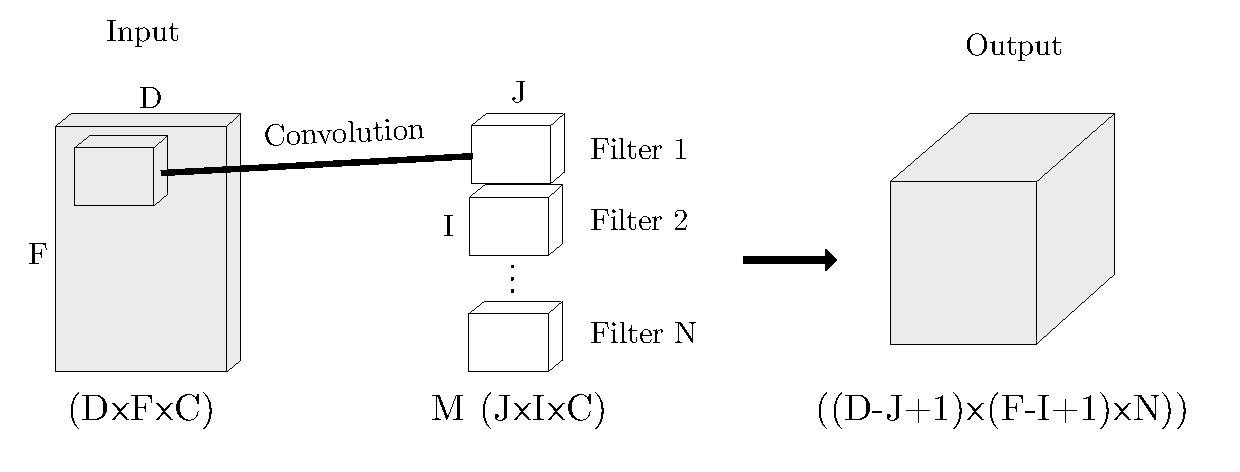
\includegraphics[width=\columnwidth]{Chapters/08_Analysis_CountNet/figures/conv.pdf}
% \caption{Illustrative diagram to show the convolution operation in
% convolution layers of CNN.\@ We consider N different local filters each
% of size \(J\times I\)}%
% \label{fig:conv}
% \end{figure}

% * good for temporal dependencies.
% * State-of-the-art speech recognition, NLP, diarization
% A recurrent neural network (RNN) layer is very similar to a fully connected network, except that RNN applies the same set of weights \(\mathbf{A}\) recursively over an input sequence.
% While convolutional layers excel in capturing local structures, RNNs can detect structure in sequential data of arbitrary length. %have an internal memory of infinite length of the past input sequence history.
% This makes it ideal to model time series, however, in practice, the temporal context learnt is limited to only a few time instances, because of the vanishing gradient problem~\cite{Hochreiter98}.
%
% To alleviate this problem, forgetting factors (also called gating) were proposed.
% One of the most popular gated recurrent cells is the Long Short-Term Memory (LSTM)~\cite{Hochreiter97} cell.
% Its effectiveness has been proven in various applications and LSTMs are the state-of-the-art approach for speech recognition~\cite{Graves13} and singing voice detection~\cite{Leglaive15}~\footnote{For a deeper mathematical background of LSTMs, due to space constraints, the reader is referred to the aforementioned papers.}.
% For a given input of dimensions \(D \times F \times C\), the output of a recurrent layer is either only the last step of dimension \(1 \times A\) or the full sequence \(D \times A\).
% The latter is useful to stack multiple LSTMs or to apply temporal max pooling of the sequence.

\subsubsection{Convolutional Recurrent Neural Network (CRNN)}%
% * Combination of CNN and Recurrent
Recently, a combination of convolutional and recurrent layers were proposed for audio-related tasks~\cite{sainath15, amodei16, Choi17, cakir17}.

The main motivation to stack these layers is to combine the benefits of convolutional layers with those of recurrent architectures, namely the benefit of convolutional layers in aggregating local features with the ability of recurrent layers to model long-term temporal data.

There are different ways to stack CNNs and RNNs to form a CRNN architecture.
In our application the motivation is to aggregate local time-frequency features coming from the output convolutional neural network and use the LSTM layer to model long temporal structures.
As the output of a CNN layer is a 3D volume \(D \times F \times C\) and the input of a recurrent layer only takes a 2D sequence, the dimension would need to be reduced. Naturally, the time dimension would need to be kept, therefore the channel dimension \(C\) is stacked with the frequency dimension \(F\) resulting in a \(D \times F \cdot C\) output.
% \begin{figure}[t]
% \centering
% 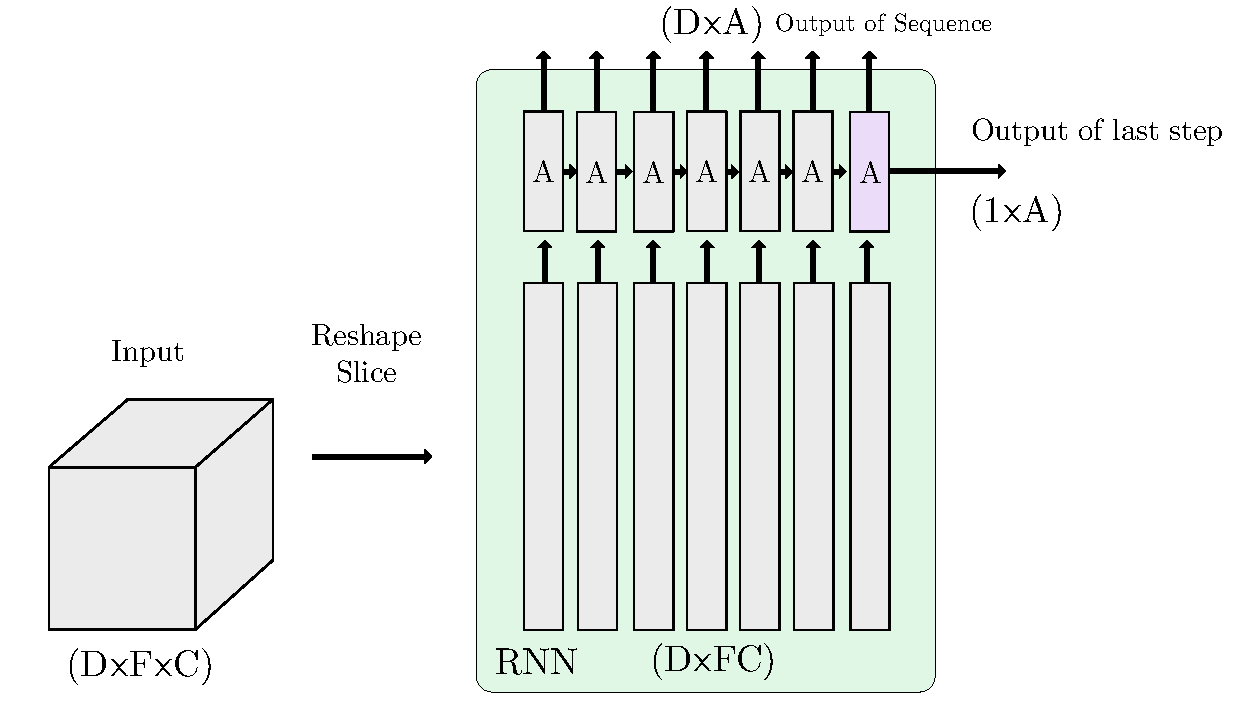
\includegraphics[width=\columnwidth]{Chapters/08_Analysis_CountNet/figures/crnn.pdf}
% \caption{Illustrative diagram to show the stacking of the output of a convolution layer into a recurrent layer with \(A\) hidden nodes per memory cell.}%
% \label{fig:crnn}
% \end{figure}

\subsubsection{Full-band Convolutional Neural Networks (F-CNN)}%
% * using full frequency band filters.
% * Very few Parameters, easy to train.
Architectures where filters span the full frequency range and therefore apply convolution in temporal direction only, have already been successfully deployed in speech~\cite{amodei16} and music application~\cite{Choi17, Pons16, Dieleman14}).
Our motivation here is that the activity of speakers happen over wide frequency ranges and a count (unlike in counting objects in images) cannot be split into sub counts.
The full-band kernel configuration only affects the first hidden layer, as in consecutive outputs all frequency bands are squashed down to one single frequency band using ``valid'' convolutions.
This is computationally very efficient, because it reduces the middle layer's dimensionality of the network significantly due to this aggregation.
To further optimize the performance of the network, we applied a hyper-parameter optimization technique using Tree-structured Parzen Estimator (TPE)~\cite{bergstra11}.
We used a search space of several hyper-parameters as shown in Table~\ref{tab:fcnnhyper} and set the maximum number of evaluations to 200.

\begin{table}
  \caption{Parameter Optimization of F-CNN Model through hyper-parameter search. Bold hyper-parameters were found optimal.}%
  \label{tab:fcnnhyper}
  \centering
\begin{tabular}{lll}
  \toprule
  Layer               & Parameters        & Value Range \\
  CNN 1               & Feature Maps      & \( \{16, \mathbf{32}, 64\} \) \\
  CNN 1               & Filter Length     & \( \{\mathbf{3}, 5, 7\} \) \\
  Pooling 1           & Pooling Length    & \( \{1, \mathbf{2}, 4\} \) \\
  CNN2                & Feature Maps      & \( \{16, \mathbf{32}, 64\} \) \\
  CNN2                & Filter Length     & \( \{\mathbf{3}, 5, 7\} \) \\
  Pooling 2           & Pooling Length    & \( \{1, 2, 4\} \) \\
  \midrule
  CNN 3               & Presence of Layer & \( \{\mathbf{Yes}, No\} \) \\
  CNN 3               & Feature Maps      & \( \{16, 32, \mathbf{64}, 128\} \) \\
  CNN 3               & Filter Length     & \( \{\mathbf{3}, 5, 7\} \) \\
  Pooling 3           & Pooling Length    & \( \{1, \mathbf{2}, 4\} \) \\
  \midrule
  Fully Connected 1   & Hidden Unit       & \( \{64, \mathbf{128}\} \) \\
  Dropout 1           & Dropout Percentage& \( [0.1, \mathbf{0.2}, 0.5] \) \\
  Fully Connected 2   & Hidden Unit       & \( \{32, \mathbf{48}\} \) \\
  Dropout 2           & Dropout Percentage& \( [0.1, \mathbf{0.2}, 0.5] \) \\
  \bottomrule
  \end{tabular}
\end{table}

The results are in agreement with the findings in~\cite{schluter16} where small filter kernels of size 3 outperformed larger kernels. Also, it can be seen from the results, that increasing the number of feature maps of the convolutional layers does not necessarily increase the performance.

\subsubsection{Full-Band Convolutional Recurrent Neural Networks (F-CRNN)}%
% * Also add recurrent.
Similarly to \emph{CRNN} and to the Deep Speech 2 implementation~\cite{amodei16}, we added an LSTM recurrent layer to the output of the last convolutional layer.
Since each filter output is only of dimension one, an additional flattening as in \emph{CRNN} is not required.

\subsection{Output Activation Functions for Count Estimation}%
\label{ssec:objectives}
% The count estimation problem can be addressed using three different strategies.
For each of the decision functions a suitable output activation and loss is used.

% Reference image object counting networks.
% * Describe matching loss functions in detail.
% Describe the DNN networks output layers very shortly

% * Classification+Softmax
\subsubsection{Classification}
For \emph{classification}, the output is required to be one-hot-encoded so that the output is of dimension \(y \in \mathbb{B}^{L + 1}\), where \(L\) is the maximum number of concurrent speakers to be expected.
In the final layer of the network, a softmax activation function is used with the cross entropy function as the loss.
% to perform classification:
% \begin{equation}
%   f_j(z) = \frac{e^{z_j}}{\sum_k e^{z_k}}
% \end{equation}
% The softmax activation function generates the posterior probability for each of the \(L + 1\) classes, by squashing the output of the last layer to values between 0 and 1.
% The categorical cross entropy is used to generate the loss where \(p\) is the correct probability and \(u\) is the amount generated by model:
%
% \begin{equation}
%   E = \sum p(x) \log(u)
% \end{equation}

% * Regression+MSE
\subsubsection{Gaussian Regression}
For the Gaussian regression model, the final output layer is of dimension \(y \in \mathbb{R}^{1}\).
The output layer nodes have linear activation, and mean squared error is used as the loss function.
% An activation function is not applied, the output is therefore linear.
% For training we use the mean squared error (MSE) function
%
% \begin{equation}
%   E = \sum \left|k-u\right|^{2}
% \end{equation}.
%
% Using the MSE can be interpreted as being derived from the negative log likelihood of normal distribution.
% So when we use MSE, we estimate the mean parameter of Normal distribution (output of the model) that is most likely to generate our data.

% * Regression+Poisson Loss
\subsubsection{Poisson Regression}
For the Poisson regression, the likelihood of parameter \(\lambda \) given the true count \(\cardinality \) is computed by the negative log likelihood loss \(E = \sum \lambda - \cardinality * \log(\lambda + eps)\). The output layer activation is the exponential function.

%
\begin{figure*}[tb]
\centering
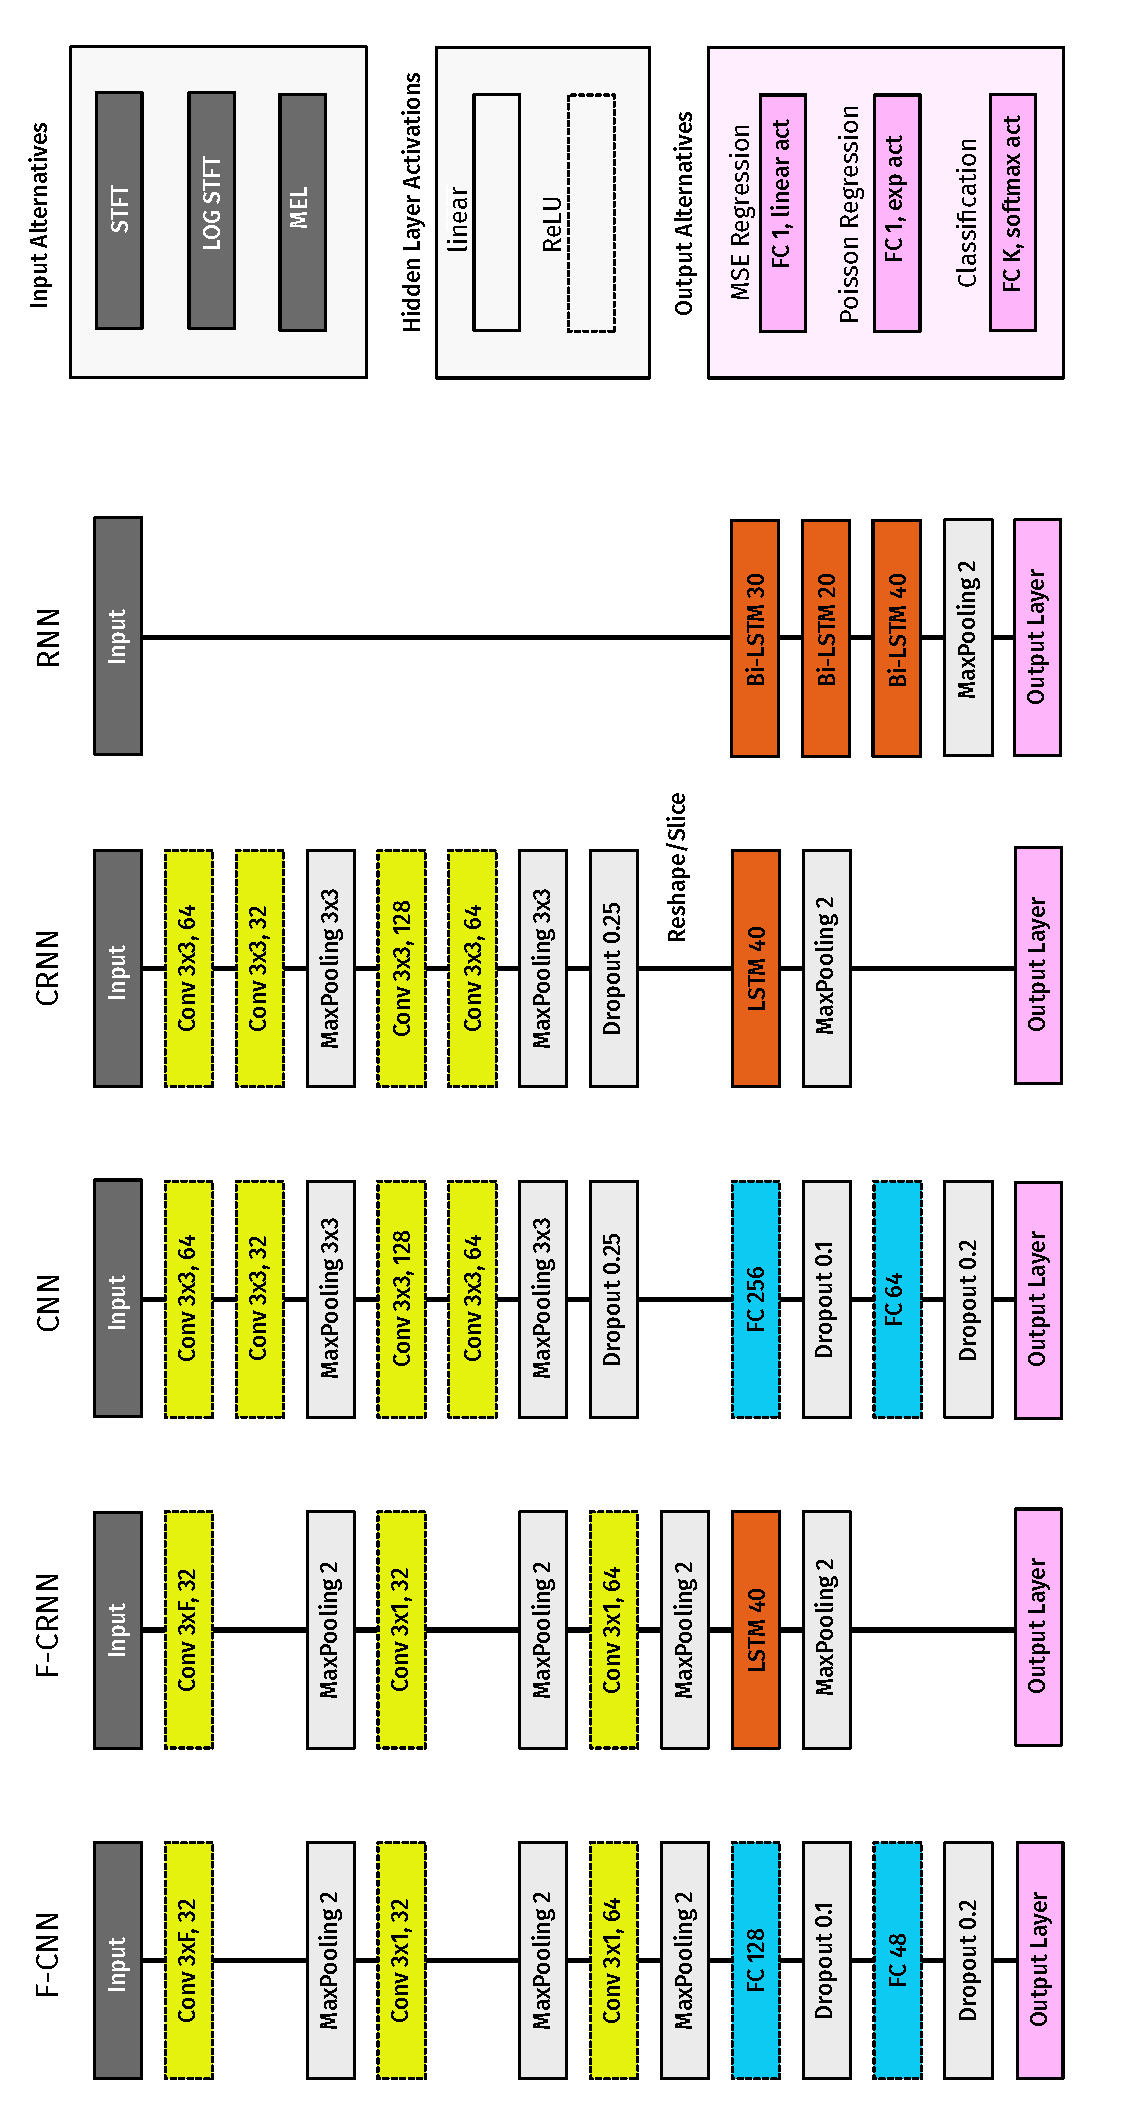
\includegraphics[width=0.9\textwidth]{Chapters/08_Analysis_CountNet/figures/networkoverview.pdf}
\caption{Overview of the proposed Architectures.}%
\label{fig:networkoverview}%
\end{figure*}

%!TEX root = ../stoeter_sourcecount.tex
\section{Training}%
\label{sec:training}

To successfully train and evaluate the proposed DNNs, due to the number of parameters, a large amount of training data is required.
In this section, we introduce relevant speech corpora and describe how the training dataset was assembled.

\subsection{Speech Corpora and Annotations}%
\label{ssec:corpus}
% * Libri Speech
% * Describe the used VAD
To date, many available speech datasets contain recordings where only a single speaker is active.
Datasets that include overlapped speech segments, either lack accurate annotations because the annotation of speech onsets and offsets in mixtures is cumbersome for humans as shown in Section~\ref{sec:introduction} or lack a controlled auditory environment such as in TV/broadcasting scenarios~\cite{Gravier12}.
Since a realistic dataset of fully overlapped speakers is not available, we chose to generate synthetic mixtures.
We recognize that in a simulated ``cocktail-party'' environment, mixtures lack the conversational aspect of human communication but provide a controlled environment which helps to understand how a DNN solves the count estimation problem.
As we aim for a speaker independent solution, we selected a speech corpus with preference to a high number of different speakers instead of the number of utterances, thus increasing the number of unique mixtures.
We selected \emph{LibriSpeech clean-360}\ \cite{panayotov15} which includes 363 hours of clean speech of English utterances from 921 speakers (439 female and 482 male speakers) sampled at 16 kHz.
% Compared to \emph{LibriSpeech}, \emph{TIMIT} is of lower recording quality and \emph{THCHS} represents mandarin speech.
% \par
% As revealed in Equation~\ref{eq:definition_k}, the maximum number of concurrent speakers \(cardinality\) requires annotation of the activity of each individual speaker.
% Even though many corpora come with word and phonemes annotation, they often are not consistent across different corpora.
% We therefore generated annotations based on a voice activity detection algorithm (VAD). As we rely on a robust VAD estimate, we found the implementation from the \emph{Chromium Web Browser} as part of the WebRTC Standard~\footnote{WebRTC 1.0: Real-time Communication Between Browsers W3C Editor's Draft 05 June 2017} to yield good results.
In the further course of this work (see Section~\ref{sec:evaluation}), we also present the results from test sets of two other datasets as listed in Table~\ref{tab:corpora}.
Furthermore, we included non-speech examples from the TUT Acoustic Scenes dataset~\cite{Mesaros16} in our training data to avoid using zero input samples for \(\cardinality = 0\) to increase the robustness against noise.

% \subsection{Training Dataset}%
% \label{ssec:train}
%
% To generate a single training sample, a tuples of speech mixtures and their ground truth speaker count \(\cardinality \), we draw a unique set of \(\cardinality \) speakers from the corpus.
% For each of the speakers we then select a random utterance, resampled to 16 kHz sampling rate and apply VAD.\@
% The VAD method was configured using default parameters using a hop size of 10~ms.
% Further, the VAD estimate was used to remove silence in the beginning and the end of an utterance recording.
% In the next step, more utterances from the same speaker are drawn from the corpus until the desired duration is reached.
% Both, the audio recording and the VAD annotation of each utterance is concatenated.
% The procedure is repeated for all speaker so that \(\cardinality \) time domain signals are created.
% Signals are mixed according to Equation~\ref{eq:mixing_model} and peak normalised to avoid clipping.
% Mixtures are then transformed to a time-frequency matrix \(X \in D \times F\).
% The VAD matrix \(v_{nl}\) is upsampled in temporal direction using nearest neighbour interpolation to match \(D\).
% The ground truth output \(\cardinality \) is then computed based on Equation~\ref{eq:definition_k}.
% \par
% We follow the proposal of~\cite{wang15} and include non-speech examples in our training data to avoid using zero input samples for \(\cardinality = 0\) and also to increase the robustness against noise.
% We used the TUT Acoustic Scenes dataset~\cite{Mesaros16} to create training samples using the same procedure as described above.
% As environmental sounds could include speech, we omitted obvious subsets such as \texttt{cafe/restaurant}, \texttt{grocery store} and \texttt{metro station}.
% Additionally we used the VAD to verify if any sample contains speech.
\begin{table}
  \centering
  \caption{Overview of speech corpora used in this work.}%
\label{tab:corpora}
\begin{tabular}{llrrr}
  \toprule
  & & \multicolumn{3}{c}{Number of Speakers} \\
  \cmidrule(r){3-5}
  Name & Language &  Train & Valid. & Test\\
  \midrule
  LibriSpeech~\cite{panayotov15} & English & 921 & 40 & 40 \\
  TIMIT~\cite{TIMIT93} & English & 462 & 24 & 168 \\
  THCHS~\cite{THCHS15} & Mandarin & 30 & 10 & 10 \\
  \bottomrule
  \end{tabular}
\end{table}

\par
A single training tuple \( \left\{\mathbf{X}, k\right\} \) is generated by a synthetic speech mixture and their ground truth speaker count \(\cardinality \).
The mixtures are formed from random utterances of different speakers where silence in the beginning and end was removed to increase the overlap within one segment.
In fact, our method to generate synthetic samples results in an average overlap for \(k=2\) of 85\% and for \(k=10\) of 55\% (based on 5s segments).
This procedure is similar to~\cite{mesaros17} used to label the data.
Signals are mixed according to Equation~\ref{eq:mixing_model}, peak normalized and then transformed to a time-frequency matrix \(X \in D \times F\).
Based on a voice activity detection algorithm (VAD), we used an implementation based on the WebRTC Standard~\cite{webrtc} where we computed the ground truth output \(\cardinality \) via Equation~\ref{eq:definition_k}.
All samples are normalized to the average Euclidean norm of \(duration\) frames to be robust against gain variations as proposed by~\cite{uhlich15}.
Furthermore, the data was scaled to zero mean and unit standard deviation across the frequency dimension \(F\) over the full training data.
Scaling parameters were saved for validation and test.
For a more detailed description of the data set, the reader is referred to~\cite{stoeter17}.

% \subsubsection{Standardization, Normalization}%
% \label{ssec:norm}
%
% As our application more closely relates to source separation we want our trained DNN system to be robust against gain variations.
% We therefore find it important that the DNN can not leverage the gain factors of the mixture.
% We found that the averaged energy of one bin across \(duration\) already is a solid indicator for the number of speakers.
% In fact, in early experiments of the methods described in~\cite{sayoud10, andrei15} we were only able to reproduce their results when no normalization was applied.
% To accommodate these findings, we normalize \(\mathbf{X}\) to the average Euclidean norm of \(duration\) frames as proposed by~\cite{Uhlich15}.
% Additionally, as common in machine learning, we scale the normalised input representation so that the feature dimension \(F\) have zero mean and unit variance/standard deviation across the whole training dataset (Standardization).

\subsection{Training Procedure}%
\label{ssec:parameters}
% * Optimizer
% other things
% To train each network we use Poisson sampling to balance the number of samples \(T_{ \cardinality}\) for each \(\cardinality \).
For all experiments we chose a medium sized training dataset of \(\cardinality \in \textrm{\{0, \ldots, 10\}}\) forming a total of \(T_{\textrm{train}} = 20.020\) mixtures  (1820 per \(k\)), each containing 10 seconds of audio, resulting in 55.55 hours of training material.
For each sample fed into the network, we select a random excerpt of duration \(D\) from each mixture. If not stated otherwise, \(D=5\)~seconds.
That way, for each epoch, the network is seeing slightly different samples, reducing the number of redundant samples and thus helping to speed up the stochastic gradient based training process.
\footnote{Note that for the validation and testing, excerpts are fixed.}
A similar training procedure is detailed in~\cite{schluter16, stoeter17}.
Each architecture is trained using the ADAM optimizer~\cite{kingma14} (learning rate: \(1 \cdot 10^{-3}\), \(\beta_1=0.9\), \(\beta_2=0.999\), \(\epsilon=1 \cdot 10^{-8}\)) using mini-batches of size 32.
Our training procedure verifies that all samples within a batch are from a different set of speakers.
In addition to the training dataset, we created a fully separated validation dataset of \(T_{\textrm{valid}} = 5720\) samples using a different set of speakers from \emph{LibriSpeech dev-clean}.
Early stopping (\(patience = 10\)) is applied by monitoring the validation loss to reduce the effect of overfitting.
% As we are interested in evaluating different input durations, we need to accommodate this our training procedure where we, instead of using the full duration of one input sample, may select an excerpt of duration \(D\).
% Now instead iterating with hop size of 1 resulting in many redundant (slightly shifted) samples, we instead randomly select the offset of this excerpt for each sample.
% This procedure verifies that all samples within a batch are from different speakers.
% After every epoch the offsets are being reset so that each epoch is seeing slightly different samples (in different order) of the same training dataset.
% Note that this is not the case for the evaluation and test dataset where the offsets are fixed using an initial seed.
% We found this procedure (also used in~\cite{schluter16}) help to speed up the stochastic gradient based training process.
% Additionally it allows us to evaluate on different excerpt durations \(D\), while keeping the training dataset fixed.
Training never exceeded more than 50 epochs.
\par
We used the Keras~\cite{chollet2015keras} framework and trained on multiple instances of Nvidia GTX 1080 GPUs.

%!TEX root = ../stoeter_sourcecount.tex
\section{Model Selection}%
\label{sec:hyperparameters}
% Describe popular Input representations and why MFCCs are not used in
% experiments, MEL  STFT, LOG STFT
%
% * All mixtures have the same 0dB SNR to all others
% * Trained on 20.020 Libri Speech Mixtures
% * Number Speakers [0, 1, 2, ..., 10]
% * Temporal Context (5s)
% * Different Input Representations (STFT 400, MEL40, log(STFT + 1)))
% * Different Output Objectives (classification, regression, p-regression)
%
% * --> Fix Input Representation to STFT because of little influence
% * --> Fix Output Objective to Classification for best overall performance

In this section, we evaluate three configurations of our proposed architectures, introduced in Section~\ref{sec:supervised_learning}.
Besides the architecture, we investigate different input representations as well as the three proposed output distributions (see Section~\ref{sec:problem_formulation}).
The goal of this is to determine the effect of these parameters and fix them to select a final trained network (model) based on these parameters.
\par
% maybe move this down to "model comparison?"
To allow for a controlled test environment and at the same time limit the number of training iterations, we fix certain parameters:
In this experiment, the level of the speakers was adjusted before mixing such that they have equal power.\@
Furthermore, the input duration \(D\) was fixed to five seconds.
For all experimental parameters, we repeated the training three times with different random seeds for each run and report averaged results to minimize random effects caused by early stopping.
We used the \emph{LibriSpeech} dataset for both training and validation and
performed evaluation of all models on \(T_{\textrm{test}} = 5720\) unique and unseen speaker mixtures from \emph{LibriSpeech test-clean} set with \(k_{\max} = 10\).
\par
% \subsection{Input Representations}
% Up to date, most discriminative models for speech applications rely on  time-frequency (TF) magnitude representations.
% This is because, compared to raw time-domain models, TF models allow for faster training due to less data redundancy leading to generally fewer trainable parameters or shorter training duration.
Several well-established input representations were evaluated in~\cite{stoeter17} such as (linear or logarithmically scaled) short-time Fourier transform (STFT), Mel filter bank outputs (MEL), Mel Frequency Cepstral Coefficients (MFCC) representations, typically chosen for speech applications.

% \begin{table}
% \caption{Speech related Input representations}
% \label{tab:inputrep}
%   \centering
% \begin{tabular}{rll}
% \toprule
% References & Task & Representation \\
% \midrule
% \cite{geiger13, hagerer17} & Overlap Detection/VAD & MFCC \\
% \cite{Graves13, sainath15, marchi17} & ASR & MEL \\
% \cite{amodei16} & ASR & STFT \\
% \cite{schluter15, schluter16} & Singing Voice AD & \(\log(1 + \mathbf{X})\) \\
% \bottomrule
% \end{tabular}
% \end{table}

% As for the task of estimating the number of speakers, we assume that a fine frequency resolution is needed to discriminate time-frequency bins with overlapped speech segments from those that only belong to a single speaker.
Even though MFCCs are used in related tasks and are included in our baseline evaluations, they are known to perform poorly when used in CNNs~\cite{Seltzer13}.
This is why we decided to not to use the MFCCs as an input for the proposed architectures.
The remaining input representations are identical to those listed in~\cite{stoeter17}:

\noindent\textbf{1) STFT}: magnitude of the Short-time Fourier transform computed using Hann-windows.
A frame length of 25~ms has been used.
The resulting input is \(X \in \mathbb{R}^{500 \times 201}\).\\
\textbf{2) LOGSTFT}: logarithmically scaled magnitudes from STFT representation using \(\log(1 + STFT)\).
The resulting input is \(X \in \mathbb{R}^{500 \times 201}\).\\
\textbf{3) MEL}: compute mapping from the STFT output directly onto Mel basis using 40 triangular filters.
The resulting input is \(X \in \mathbb{R}^{500 \times 40}\).
\par
Before feature transformation, all input files were re-sampled to 16 kHz sampling rate. All features are computed using a hop size of 10~ms.

\subsection{Metric}%
\label{ssec:metrics}

Whereas the intermediate output \(y\) is treated as either a classification or a regression problem (see Section~\ref{sec:problem_formulation}) we evaluate the final output \(\cardinality \) as a discrete regression problem.
We, therefore, employ the mean absolute error (MAE) which is also commonly used for other count related tasks (c.f.~\cite{zhang15, Rezatofigh16}).
Since the MAE depends on the true count \(\cardinality \), we also present the MAE per class as:

\begin{equation}
  \mbox{MAE}(k) = \frac{1}{T_{\textrm{test}}} \sum_{t=1}^{T_\textrm{test}}\left| \hat{k} - k \right|.
\end{equation}

which is then averaged

\begin{equation}
  \mbox{MAE} = \frac{1}{k_{\max}} \sum_{k=0}^{k_{\max}} \mbox{MAE}(k).
\end{equation}

% * Mean Speaker Count Distance
% * Accuracy
% * Accuracy +/- 1
% * Response

\subsection{Model Comparison}%
\label{ssec:model_comparsion}


\begin{figure*}
\centering
\subcaptionbox[by feature representations.]{%
    by feature representations.%
    \label{fig:ssec:exp_fixed_gains/A}%
}
[%
    \textwidth % width of caption
]%
{%
  % This file was created by matplotlib2tikz v0.6.13.
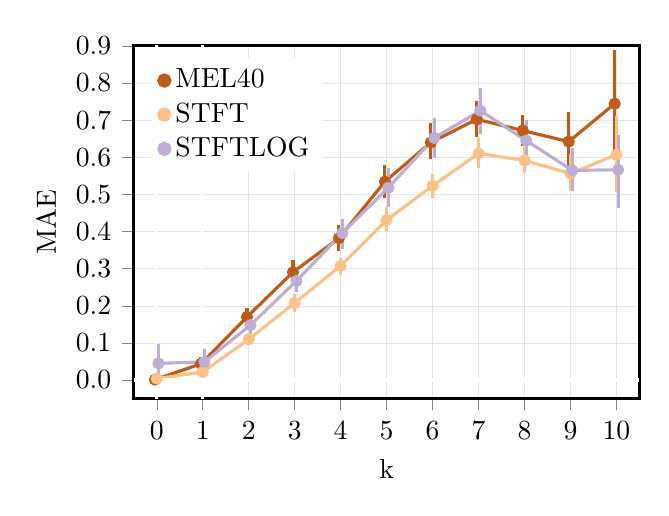
\begin{tikzpicture}

% colors from colorbrewer Set3
\definecolor{color0}{rgb}{0.917647058823529,0.917647058823529,0.949019607843137}
\definecolor{color1}{RGB}{191,91,23}
\definecolor{color3}{RGB}{190,174,212}
\definecolor{color2}{RGB}{253,192,134}

\begin{axis}[
xlabel={k},
ylabel={MAE},
width=0.66\textwidth,
height=0.5\textwidth,
xmin=-0.5, xmax=10.5,
ymin=-0.05, ymax=0.9,
ytick={-0.1,0,0.1,0.2,0.3,0.4,0.5,0.6,0.7,0.8,0.9},
yticklabels={0.0,0.0,0.1,0.2,0.3,0.4,0.5,0.6,0.7,0.8,0.9},
xtick distance=1,
tick align=outside,
tick pos=left,
ymajorgrids,
xmajorgrids,
grid style={line width=.1pt, draw=gray!20},
major grid style={line width=.2pt,draw=gray!20},
axis line style={black},
legend style={at={(0.03,0.97)}, anchor=north west, draw=none, fill==gray!0},
legend cell align={left},
legend entries={{MEL40},{STFT},{STFTLOG}}
]
\addplot [only marks, draw=color1, fill=color1, colormap/blackwhite]
table{%
x                      y
-3.750000000000001e-02 +1.282051285115891e-03
+9.625000000000000e-01 +4.378956559182671e-02
+1.962500000000000e+00 +1.698966412812240e-01
+2.962500000000000e+00 +2.904593644946708e-01
+3.962500000000000e+00 +3.819121458168999e-01
+4.962500000000000e+00 +5.342699044052212e-01
+5.962500000000000e+00 +6.399449048893949e-01
+6.962500000000000e+00 +7.022138688498571e-01
+7.962500000000000e+00 +6.717410322614437e-01
+8.962500000000000e+00 +6.421099899821276e-01
+9.962500000000000e+00 +7.441498321916922e-01
};
\addplot [line width=2.00pt, color1, forget plot]
table {%
-0.0375 0.00128205128511589
0.9625 0.0437895655918267
1.9625 0.169896641281224
2.9625 0.290459364494671
3.9625 0.3819121458169
4.9625 0.534269904405221
5.9625 0.639944904889395
6.9625 0.702213868849857
7.9625 0.671741032261444
8.9625 0.642109989982128
9.9625 0.744149832191692
};
\addplot [line width=2.00pt, color1, forget plot]
table {%
-0.0375 0.0002991452993443
-0.0375 0.00290598291171611
};
\addplot [line width=2.00pt, color1, forget plot]
table {%
0.9625 0.0292021391029433
0.9625 0.0628356254969424
};
\addplot [line width=2.00pt, color1, forget plot]
table {%
1.9625 0.148319336806491
1.9625 0.1932881148387
};
\addplot [line width=2.00pt, color1, forget plot]
table {%
2.9625 0.260852964485001
2.9625 0.322079899352019
};
\addplot [line width=2.00pt, color1, forget plot]
table {%
3.9625 0.348403317338685
3.9625 0.418488374525981
};
\addplot [line width=2.00pt, color1, forget plot]
table {%
4.9625 0.490396980724153
4.9625 0.580383148183019
};
\addplot [line width=2.00pt, color1, forget plot]
table {%
5.9625 0.59489899164649
5.9625 0.690870064470585
};
\addplot [line width=2.00pt, color1, forget plot]
table {%
6.9625 0.654216791062228
6.9625 0.75059524217121
};
\addplot [line width=2.00pt, color1, forget plot]
table {%
7.9625 0.629482719495514
7.9625 0.712939632123146
};
\addplot [line width=2.00pt, color1, forget plot]
table {%
8.9625 0.5712637464472
8.9625 0.720740745223197
};
\addplot [line width=2.00pt, color1, forget plot]
table {%
9.9625 0.603217593893058
9.9625 0.889956860029537
};
\addplot [only marks, draw=color2, fill=color2, colormap/blackwhite]
table{%
x                      y
+0.000000000000000e+00 +4.017094149429383e-03
+1.000000000000000e+00 +2.165466058294658e-02
+2.000000000000000e+00 +1.097760553809459e-01
+3.000000000000000e+00 +2.075775420503098e-01
+4.000000000000000e+00 +3.075366057808496e-01
+5.000000000000000e+00 +4.309067676908769e-01
+6.000000000000000e+00 +5.230027550672368e-01
+7.000000000000000e+00 +6.100250622981175e-01
+8.000000000000000e+00 +5.915135611073551e-01
+9.000000000000000e+00 +5.562738505022561e-01
+1.000000000000000e+01 +6.068181814770105e-01
};
\addplot [line width=2.00pt, color2, forget plot]
table {%
0 0.00401709414942938
1 0.0216546605829466
2 0.109776055380946
3 0.20757754205031
4 0.30753660578085
5 0.430906767690877
6 0.523002755067237
7 0.610025062298117
8 0.591513561107355
9 0.556273850502256
10 0.60681818147701
};
\addplot [line width=2.00pt, color2, forget plot]
table {%
0 0.00141025642932265
0 0.00777884649395501
};
\addplot [line width=2.00pt, color2, forget plot]
table {%
1 0.015104780559566
1 0.0292981881977767
};
\addplot [line width=2.00pt, color2, forget plot]
table {%
2 0.0935389754212398
2 0.126616063651554
};
\addplot [line width=2.00pt, color2, forget plot]
table {%
3 0.184214762288727
3 0.232517668003831
};
\addplot [line width=2.00pt, color2, forget plot]
table {%
4 0.283712317184782
4 0.329804048656288
};
\addplot [line width=2.00pt, color2, forget plot]
table {%
5 0.401557044723647
5 0.465348019600485
};
\addplot [line width=2.00pt, color2, forget plot]
table {%
6 0.490907942142724
6 0.554963269541031
};
\addplot [line width=2.00pt, color2, forget plot]
table {%
7 0.571706349037544
7 0.650759191716972
};
\addplot [line width=2.00pt, color2, forget plot]
table {%
8 0.557388451102525
8 0.628085083916509
};
\addplot [line width=2.00pt, color2, forget plot]
table {%
9 0.510563413293006
9 0.60849158311509
};
\addplot [line width=2.00pt, color2, forget plot]
table {%
10 0.507567340790322
10 0.711869740708408
};
\path [draw=white, fill opacity=0] (axis cs:0,-0.0552693502854651)
--(axis cs:0,0.934967631949299);

\path [draw=white, fill opacity=0] (axis cs:1,-0.0552693502854651)
--(axis cs:1,0.934967631949299);

\path [draw=white, fill opacity=0] (axis cs:-0.5,0)
--(axis cs:10.5,0);

\path [draw=white, fill opacity=0] (axis cs:-0.5,1)
--(axis cs:10.5,1);

\addplot [only marks, draw=color3, fill=color3, colormap/blackwhite]
table{%
x                      y
+3.750000000000001e-02 +4.491453003381084e-02
+1.037500000000000e+00 +4.894127914890618e-02
+2.037500000000000e+00 +1.479328153983824e-01
+3.037500000000000e+00 +2.669022376087070e-01
+4.037500000000000e+00 +3.958656320969263e-01
+5.037500000000000e+00 +5.179225227638933e-01
+6.037500000000000e+00 +6.520202012977215e-01
+7.037500000000000e+00 +7.256892264536648e-01
+8.037500000000000e+00 +6.448818897898534e-01
+9.037500000000000e+00 +5.645342315434071e-01
+1.003750000000000e+01 +5.662037049329240e-01
};
\addplot [line width=2.00pt, color3, forget plot]
table {%
0.0375 0.0449145300338108
1.0375 0.0489412791489062
2.0375 0.147932815398382
3.0375 0.266902237608707
4.0375 0.395865632096926
5.0375 0.517922522763893
6.0375 0.652020201297722
7.0375 0.725689226453665
8.0375 0.644881889789853
9.0375 0.564534231543407
10.0375 0.566203704932924
};
\addplot [line width=2.00pt, color3, forget plot]
table {%
0.0375 0.00563675216719425
0.0375 0.0978333334729233
};
\addplot [line width=2.00pt, color3, forget plot]
table {%
1.0375 0.0240973587901605
1.0375 0.083095393889988
};
\addplot [line width=2.00pt, color3, forget plot]
table {%
2.0375 0.119852497411666
2.0375 0.180880703087784
};
\addplot [line width=2.00pt, color3, forget plot]
table {%
3.0375 0.236119944983176
3.0375 0.298233213870577
};
\addplot [line width=2.00pt, color3, forget plot]
table {%
4.0375 0.354053618227044
4.0375 0.434679154426463
};
\addplot [line width=2.00pt, color3, forget plot]
table {%
5.0375 0.46628033370452
5.0375 0.5704150723004
};
\addplot [line width=2.00pt, color3, forget plot]
table {%
6.0375 0.599070247832217
6.0375 0.705386820743399
};
\addplot [line width=2.00pt, color3, forget plot]
table {%
7.0375 0.663815792690194
7.0375 0.786649962138935
};
\addplot [line width=2.00pt, color3, forget plot]
table {%
8.0375 0.588227250151147
8.0375 0.700395887889496
};
\addplot [line width=2.00pt, color3, forget plot]
table {%
9.0375 0.508768798929406
9.0375 0.623634119981668
};
\addplot [line width=2.00pt, color3, forget plot]
table {%
10.0375 0.464126683435331
10.0375 0.659747474216276
};
\end{axis}

\end{tikzpicture}

}%
\hspace{0.2\textwidth} % seperation
\subcaptionbox[by output distribution.]{%
    by output distribution.%
    \label{fig:ssec:exp_fixed_gains/A}%
}
[%
    \textwidth % width of caption
]%
{%
  % This file was created by matplotlib2tikz v0.6.13.
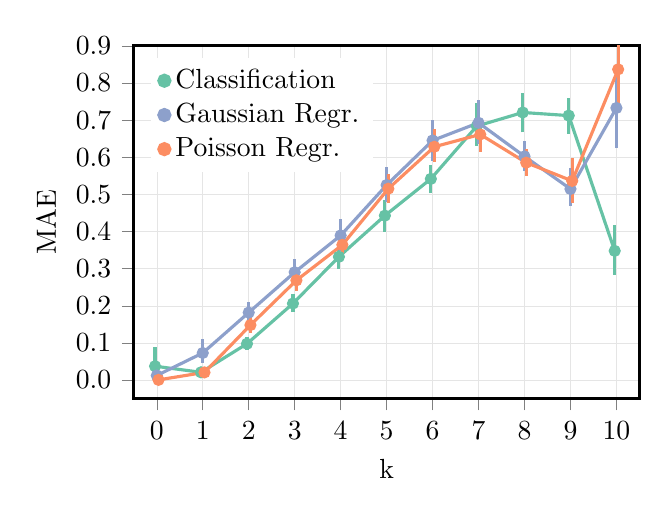
\begin{tikzpicture}

\definecolor{color0}{rgb}{0.917647058823529,0.917647058823529,0.949019607843137}
\definecolor{color1}{RGB}{102,194,165}
\definecolor{color3}{RGB}{252,141,98}
\definecolor{color2}{RGB}{141,160,203}

\begin{axis}[
xlabel={k},
ylabel={MAE},
width=0.66\textwidth,
height=0.5\textwidth,
xmin=-0.5, xmax=10.5,
ymin=-0.05, ymax=0.9,
ytick={-0.1,0,0.1,0.2,0.3,0.4,0.5,0.6,0.7,0.8,0.9},
yticklabels={0.0,0.0,0.1,0.2,0.3,0.4,0.5,0.6,0.7,0.8,0.9},
xtick distance=1,
tick align=outside,
tick pos=left,
ymajorgrids,
xmajorgrids,
axis line style={black},
grid style={line width=.1pt, draw=gray!20},
major grid style={line width=.2pt,draw=gray!20},
legend style={at={(0.03,0.97)}, anchor=north west, draw=none, fill==gray!0},
legend entries={{Classification},{Gaussian Regr.},{Poisson Regr.}},
legend cell align={left}
]
\addplot [only marks, draw=color1, fill=color1, colormap/blackwhite]
table{%
x                      y
-3.750000000000001e-02 +3.735042735042735e-02
+9.625000000000000e-01 +2.086880593756822e-02
+1.962500000000000e+00 +9.780361757105942e-02
+2.962500000000000e+00 +2.061248527679623e-01
+3.962500000000000e+00 +3.319121447028424e-01
+4.962500000000000e+00 +4.427415921668795e-01
+5.962500000000000e+00 +5.417355371900826e-01
+6.962500000000000e+00 +6.838345864661655e-01
+7.962500000000000e+00 +7.204724409448819e-01
+8.962500000000000e+00 +7.120987654320987e-01
+9.962500000000000e+00 +3.478956228956228e-01
};
\addplot [line width=2.00pt, color1, forget plot]
table {%
-0.0375 0.0373504273504274
0.9625 0.0208688059375682
1.9625 0.0978036175710594
2.9625 0.206124852767962
3.9625 0.331912144702842
4.9625 0.44274159216688
5.9625 0.541735537190083
6.9625 0.683834586466165
7.9625 0.720472440944882
8.9625 0.712098765432099
9.9625 0.347895622895623
};
\addplot [line width=2.00pt, color1, forget plot]
table {%
-0.0375 0.00153739316239316
-0.0375 0.0895363247863248
};
\addplot [line width=2.00pt, color1, forget plot]
table {%
0.9625 0.0127919668194717
0.9625 0.0316961362148003
};
\addplot [line width=2.00pt, color1, forget plot]
table {%
1.9625 0.0817797157622739
1.9625 0.114736218776916
};
\addplot [line width=2.00pt, color1, forget plot]
table {%
2.9625 0.182602080879466
2.9625 0.231887514723204
};
\addplot [line width=2.00pt, color1, forget plot]
table {%
3.9625 0.29969315245478
3.9625 0.365779500430663
};
\addplot [line width=2.00pt, color1, forget plot]
table {%
4.9625 0.399341209025117
4.9625 0.485740740740741
};
\addplot [line width=2.00pt, color1, forget plot]
table {%
5.9625 0.502793847566575
5.9625 0.579757805325987
};
\addplot [line width=2.00pt, color1, forget plot]
table {%
6.9625 0.631313700918964
6.9625 0.745908521303258
};
\addplot [line width=2.00pt, color1, forget plot]
table {%
7.9625 0.66682195975503
7.9625 0.773801399825022
};
\addplot [line width=2.00pt, color1, forget plot]
table {%
8.9625 0.663826038159372
8.9625 0.758792368125701
};
\addplot [line width=2.00pt, color1, forget plot]
table {%
9.9625 0.283256523569024
9.9625 0.418800505050505
};
\addplot [only marks, draw=color2, fill=color2, colormap/blackwhite]
table{%
x                      y
+0.000000000000000e+00 +1.235042760510825e-02
+1.000000000000000e+00 +7.290984498750833e-02
+2.000000000000000e+00 +1.817398789856169e-01
+3.000000000000000e+00 +2.903023165133264e-01
+4.000000000000000e+00 +3.893195516533322e-01
+5.000000000000000e+00 +5.250319321950276e-01
+6.000000000000000e+00 +6.450872368282742e-01
+7.000000000000000e+00 +6.927318334579468e-01
+8.000000000000000e+00 +6.023184604114956e-01
+9.000000000000000e+00 +5.145679036776225e-01
+1.000000000000000e+01 +7.327020216319297e-01
};
\addplot [line width=2.00pt, color2, forget plot]
table {%
0 0.0123504276051083
1 0.0729098449875083
2 0.181739878985617
3 0.290302316513326
4 0.389319551653332
5 0.525031932195028
6 0.645087236828274
7 0.692731833457947
8 0.602318460411496
9 0.514567903677623
10 0.73270202163193
};
\addplot [line width=2.00pt, color2, forget plot]
table {%
0 0.00534081213764795
0 0.0241025645566535
};
\addplot [line width=2.00pt, color2, forget plot]
table {%
1 0.0466262830175563
1 0.110413665477342
};
\addplot [line width=2.00pt, color2, forget plot]
table {%
2 0.155333763578286
2 0.211202626282142
};
\addplot [line width=2.00pt, color2, forget plot]
table {%
3 0.257034745460583
3 0.324860619132717
};
\addplot [line width=2.00pt, color2, forget plot]
table {%
4 0.34692829568353
4 0.432953272768193
};
\addplot [line width=2.00pt, color2, forget plot]
table {%
5 0.478991059346331
5 0.574425296684106
};
\addplot [line width=2.00pt, color2, forget plot]
table {%
6 0.590747243298425
6 0.699374426702658
};
\addplot [line width=2.00pt, color2, forget plot]
table {%
7 0.634959278139803
7 0.754830837696791
};
\addplot [line width=2.00pt, color2, forget plot]
table {%
8 0.562505469305648
8 0.6433584856987
};
\addplot [line width=2.00pt, color2, forget plot]
table {%
9 0.468725030223529
9 0.570103260063463
};
\addplot [line width=2.00pt, color2, forget plot]
table {%
10 0.624493893070353
10 0.840917507157558
};
% \path [draw=white, fill opacity=0] (axis cs:0,-0.0600185928210457)
% --(axis cs:0,1.00006922752411);
%
% \path [draw=white, fill opacity=0] (axis cs:1,-0.0600185928210457)
% --(axis cs:1,1.00006922752411);
%
% \path [draw=white, fill opacity=0] (axis cs:-0.5,0)
% --(axis cs:10.5,0);
%
% \path [draw=white, fill opacity=0] (axis cs:-0.5,1)
% --(axis cs:10.5,1);

\addplot [only marks, draw=color3, fill=color3, colormap/blackwhite]
table{%
x                      y
+3.750000000000001e-02 +5.128205128205128e-04
+1.037500000000000e+00 +2.060685439860293e-02
+2.037500000000000e+00 +1.480620155038760e-01
+3.037500000000000e+00 +2.685119748723989e-01
+4.037500000000000e+00 +3.640826873385014e-01
+5.037500000000000e+00 +5.153256704980842e-01
+6.037500000000000e+00 +6.281450872359963e-01
+7.037500000000000e+00 +6.613617376775270e-01
+8.037500000000000e+00 +5.853455818022747e-01
+9.037500000000000e+00 +5.362514029180696e-01
+1.003750000000000e+01 +8.365740740740741e-01
};
\addplot [line width=2.00pt, color3, forget plot]
table {%
0.0375 0.000512820512820513
1.0375 0.0206068543986029
2.0375 0.148062015503876
3.0375 0.268511974872399
4.0375 0.364082687338501
5.0375 0.515325670498084
6.0375 0.628145087235996
7.0375 0.661361737677527
8.0375 0.585345581802275
9.0375 0.53625140291807
10.0375 0.836574074074074
};
\addplot [line width=2.00pt, color3, forget plot]
table {%
0.0375 0.000170940170940171
0.0375 0.000982905982905983
};
\addplot [line width=2.00pt, color3, forget plot]
table {%
1.0375 0.0122647893473041
1.0375 0.0345797860729098
};
\addplot [line width=2.00pt, color3, forget plot]
table {%
2.0375 0.12656976744186
2.0375 0.169559646856158
};
\addplot [line width=2.00pt, color3, forget plot]
table {%
3.0375 0.240591872791519
3.0375 0.298862387122104
};
\addplot [line width=2.00pt, color3, forget plot]
table {%
4.0375 0.332558139534884
4.0375 0.39405684754522
};
\addplot [line width=2.00pt, color3, forget plot]
table {%
5.0375 0.476749680715198
5.0375 0.554259259259259
};
\addplot [line width=2.00pt, color3, forget plot]
table {%
6.0375 0.587143021120294
6.0375 0.676090449954086
};
\addplot [line width=2.00pt, color3, forget plot]
table {%
7.0375 0.614816207184628
7.0375 0.704314954051796
};
\addplot [line width=2.00pt, color3, forget plot]
table {%
8.0375 0.549119641294838
8.0375 0.623103674540682
};
\addplot [line width=2.00pt, color3, forget plot]
table {%
9.0375 0.475597081930415
9.0375 0.597627384960718
};
\addplot [line width=2.00pt, color3, forget plot]
table {%
10.0375 0.727001262626263
10.0375 0.951883417508417
};
\end{axis}

\end{tikzpicture}

}%
\hspace{0.2\textwidth} % seperation
\subcaptionbox[by feature representations.]{%
    by feature representations.%
    \label{fig:ssec:exp_fixed_gains/A}%
}
[%
    \textwidth % width of caption
]%
{%
  % This file was created by matplotlib2tikz v0.6.13.
\begin{tikzpicture}

\definecolor{color0}{rgb}{0.917647058823529,0.917647058823529,0.949019607843137}

\begin{axis}[
xlabel={k},
ylabel={MAE},
width=0.66\textwidth,
height=0.5\textwidth,
xmin=-0.5, xmax=10.5,
ymin=-0.05, ymax=0.9,
ytick={-0.1,0,0.1,0.2,0.3,0.4,0.5,0.6,0.7,0.8,0.9},
yticklabels={0.0,0.0,0.1,0.2,0.3,0.4,0.5,0.6,0.7,0.8,0.9},
xtick distance=1,
tick align=outside,
tick pos=left,
ymajorgrids,
xmajorgrids,
axis line style={black},
grid style={line width=.1pt, draw=gray!20},
major grid style={line width=.2pt,draw=gray!20},
legend entries={{F-CNN},{CNN},{F-CRNN},{CRNN},{RNN~\cite{stoeter17}}},
legend style={at={(0.03,0.97)}, anchor=north west, draw=none, fill=gray!0, font=\scriptsize},
legend cell align={left}
]
\addplot [only marks, draw=FCNN, fill=FCNN, colormap/blackwhite]
table{%
x                      y
-6.250000000000000e-02 +1.609686645533242e-02
+9.375000000000000e-01 +6.810740004287860e-02
+1.937500000000000e+00 +1.871231682694852e-01
+2.937500000000000e+00 +2.900143965558066e-01
+3.937500000000000e+00 +4.082687340469289e-01
+4.937500000000000e+00 +5.654179110829165e-01
+5.937500000000000e+00 +6.553412880013030e-01
+6.937500000000000e+00 +7.385129500517637e-01
+7.937500000000000e+00 +6.676144655364774e-01
+8.937500000000000e+00 +6.725028088197162e-01
+9.937500000000000e+00 +8.343855208151804e-01
};
\addplot [line width=2.00pt, FCNN, forget plot]
table {%
-0.0625 0.0160968664553324
0.9375 0.0681074000428786
1.9375 0.187123168269485
2.9375 0.290014396555807
3.9375 0.408268734046929
4.9375 0.565417911082917
5.9375 0.655341288001303
6.9375 0.738512950051764
7.9375 0.667614465536477
8.9375 0.672502808819716
9.9375 0.83438552081518
};
\addplot [line width=2.00pt, FCNN, forget plot]
table {%
-0.0625 0.00427350433559245
-0.0625 0.032419872278337
};
\addplot [line width=2.00pt, FCNN, forget plot]
table {%
0.9375 0.0406734335280436
0.9375 0.10157898504591
};
\addplot [line width=2.00pt, FCNN, forget plot]
table {%
1.9375 0.149366565919747
1.9375 0.233137736180939
};
\addplot [line width=2.00pt, FCNN, forget plot]
table {%
2.9375 0.254217380758762
2.9375 0.327314815066483
};
\addplot [line width=2.00pt, FCNN, forget plot]
table {%
3.9375 0.374671620453119
3.9375 0.445592879322353
};
\addplot [line width=2.00pt, FCNN, forget plot]
table {%
4.9375 0.520718039641279
4.9375 0.61367780890385
};
\addplot [line width=2.00pt, FCNN, forget plot]
table {%
5.9375 0.600531829466213
5.9375 0.715734995382986
};
\addplot [line width=2.00pt, FCNN, forget plot]
table {%
6.9375 0.673544972183909
6.9375 0.808347258480503
};
\addplot [line width=2.00pt, FCNN, forget plot]
table {%
7.9375 0.600100245278955
7.9375 0.744099954962643
};
\addplot [line width=2.00pt, FCNN, forget plot]
table {%
8.9375 0.585170224673887
8.9375 0.760961468631839
};
\addplot [line width=2.00pt, FCNN, forget plot]
table {%
9.9375 0.656660354222713
9.9375 1.02770763036244
};
\addplot [only marks, draw=CNN, fill=CNN, colormap/blackwhite]
table{%
x                      y
-3.125000000000000e-02 +1.495726509789201e-03
+9.687500000000000e-01 +1.760896459410368e-02
+1.968750000000000e+00 +1.216623599392619e-01
+2.968750000000000e+00 +2.069100901482539e-01
+3.968750000000000e+00 +2.922049940205702e-01
+4.968750000000000e+00 +4.167730962238836e-01
+5.968750000000000e+00 +5.557086000319903e-01
+6.968750000000000e+00 +5.869534927485414e-01
+7.968750000000000e+00 +5.456401261879356e-01
+8.968750000000000e+00 +5.296670419778263e-01
+9.968750000000000e+00 +6.469556705317513e-01
};
\addplot [line width=2.00pt, CNN, forget plot]
table {%
-0.03125 0.0014957265097892
0.96875 0.0176089645941037
1.96875 0.121662359939262
2.96875 0.206910090148254
3.96875 0.29220499402057
4.96875 0.416773096223884
5.96875 0.55570860003199
6.96875 0.586953492748541
7.96875 0.545640126187936
8.96875 0.529667041977826
9.96875 0.646955670531751
};
\addplot [line width=2.00pt, CNN, forget plot]
table {%
-0.03125 0.000569800578609661
-0.03125 0.00242343307596477
};
\addplot [line width=2.00pt, CNN, forget plot]
table {%
0.96875 0.0108382449495332
0.96875 0.0252510370163853
};
\addplot [line width=2.00pt, CNN, forget plot]
table {%
1.96875 0.0968938411976859
1.96875 0.149162000738605
};
\addplot [line width=2.00pt, CNN, forget plot]
table {%
2.96875 0.172551041119997
2.96875 0.243168432323684
};
\addplot [line width=2.00pt, CNN, forget plot]
table {%
3.96875 0.253718057931103
3.96875 0.335432813824626
};
\addplot [line width=2.00pt, CNN, forget plot]
table {%
4.96875 0.357010075388622
4.96875 0.480567972900403
};
\addplot [line width=2.00pt, CNN, forget plot]
table {%
5.96875 0.49686065282448
5.96875 0.629650670435721
};
\addplot [line width=2.00pt, CNN, forget plot]
table {%
6.96875 0.520739347236638
6.96875 0.652126840199934
};
\addplot [line width=2.00pt, CNN, forget plot]
table {%
7.96875 0.500136699940119
7.96875 0.588074144240187
};
\addplot [line width=2.00pt, CNN, forget plot]
table {%
8.96875 0.475188928860774
8.96875 0.57882903330265
};
\addplot [line width=2.00pt, CNN, forget plot]
table {%
9.96875 0.499768520983649
9.96875 0.791559695281866
};
\path [draw=white, fill opacity=0] (axis cs:0,-0.0642762651515782)
--(axis cs:0,1.07970686348216);

\path [draw=white, fill opacity=0] (axis cs:1,-0.0642762651515782)
--(axis cs:1,1.07970686348216);

\path [draw=white, fill opacity=0] (axis cs:-0.5,0)
--(axis cs:10.5,0);

\path [draw=white, fill opacity=0] (axis cs:-0.5,1)
--(axis cs:10.5,1);

\addplot [only marks, draw=FCRNN, fill=FCRNN, colormap/blackwhite]
table{%
x                      y
+0.000000000000000e+00 +6.346153848163752e-02
+1.000000000000000e+00 +7.218220163694986e-02
+2.000000000000000e+00 +1.653028996578414e-01
+3.000000000000000e+00 +2.925664174269669e-01
+4.000000000000000e+00 +4.153029006632313e-01
+5.000000000000000e+00 +5.485312881513033e-01
+6.000000000000000e+00 +6.603152773086178e-01
+7.000000000000000e+00 +7.562656681606015e-01
+8.000000000000000e+00 +6.770195411537229e-01
+9.000000000000000e+00 +5.510662176793674e-01
+1.000000000000000e+01 +6.087962971993969e-01
};
\addplot [line width=2.00pt, FCRNN, forget plot]
table {%
0 0.0634615384816375
1 0.0721822016369499
2 0.165302899657841
3 0.292566417426967
4 0.415302900663231
5 0.548531288151303
6 0.660315277308618
7 0.756265668160601
8 0.677019541153723
9 0.551066217679367
10 0.608796297199397
};
\addplot [line width=2.00pt, FCRNN, forget plot]
table {%
0 0.00327457266575969
0 0.152783119675935
};
\addplot [line width=2.00pt, FCRNN, forget plot]
table {%
1 0.0379811538036914
1 0.117306993108207
};
\addplot [line width=2.00pt, FCRNN, forget plot]
table {%
2 0.142825868812946
2 0.189570772423677
};
\addplot [line width=2.00pt, FCRNN, forget plot]
table {%
3 0.26108166456477
3 0.321173601928928
};
\addplot [line width=2.00pt, FCRNN, forget plot]
table {%
4 0.379186404986292
4 0.450771608875335
};
\addplot [line width=2.00pt, FCRNN, forget plot]
table {%
5 0.503400382091471
5 0.592736270459379
};
\addplot [line width=2.00pt, FCRNN, forget plot]
table {%
6 0.610785893782549
6 0.711432509583583
};
\addplot [line width=2.00pt, FCRNN, forget plot]
table {%
7 0.707322127606271
7 0.805423287159302
};
\addplot [line width=2.00pt, FCRNN, forget plot]
table {%
8 0.627726745471189
8 0.733316930837779
};
\addplot [line width=2.00pt, FCRNN, forget plot]
table {%
9 0.488881408392023
9 0.614322857952468
};
\addplot [line width=2.00pt, FCRNN, forget plot]
table {%
10 0.498625141462493
10 0.723000841983307
};
\addplot [only marks, draw=CRNN, fill=CRNN, colormap/blackwhite]
table{%
x                      y
+3.125000000000000e-02 +1.424501451631833e-03
+1.031250000000000e+00 +7.567488835640818e-03
+2.031250000000000e+00 +7.493540085798669e-02
+3.031250000000000e+00 +1.739301140378820e-01
+4.031250000000000e+00 +2.658627627782701e-01
+5.031250000000000e+00 +3.860508020218169e-01
+6.031250000000000e+00 +5.054331182119932e-01
+7.031250000000000e+00 +5.913394604825403e-01
+8.031250000000000e+00 +5.926655008150419e-01
+9.031250000000000e+00 +4.832023948219176e-01
+1.003125000000000e+01 +3.981481475209950e-01
};
\addplot [line width=2.00pt, CRNN, forget plot]
table {%
0.03125 0.00142450145163183
1.03125 0.00756748883564082
2.03125 0.0749354008579867
3.03125 0.173930114037882
4.03125 0.26586276277827
5.03125 0.386050802021817
6.03125 0.505433118211993
7.03125 0.59133946048254
8.03125 0.592665500815042
9.03125 0.483202394821918
10.03125 0.398148147520995
};
\addplot [line width=2.00pt, CRNN, forget plot]
table {%
0.03125 0.0004985754989735
0.03125 0.00270655276526948
};
\addplot [line width=2.00pt, CRNN, forget plot]
table {%
1.03125 0.00203558178730112
1.03125 0.0145546822128031
};
\addplot [line width=2.00pt, CRNN, forget plot]
table {%
2.03125 0.0569157335567367
2.03125 0.0955408415482242
};
\addplot [line width=2.00pt, CRNN, forget plot]
table {%
3.03125 0.146104894003063
3.03125 0.204166667151622
};
\addplot [line width=2.00pt, CRNN, forget plot]
table {%
4.03125 0.23291343713199
4.03125 0.2977354312345
};
\addplot [line width=2.00pt, CRNN, forget plot]
table {%
5.03125 0.348859443451997
5.03125 0.421471903264116
};
\addplot [line width=2.00pt, CRNN, forget plot]
table {%
6.03125 0.457526017299231
6.03125 0.55380509473705
};
\addplot [line width=2.00pt, CRNN, forget plot]
table {%
7.03125 0.533848510757068
7.03125 0.653164161347108
};
\addplot [line width=2.00pt, CRNN, forget plot]
table {%
8.03125 0.543070136671617
8.03125 0.643294327571819
};
\addplot [line width=2.00pt, CRNN, forget plot]
table {%
9.03125 0.423866442182048
9.03125 0.545838009867325
};
\addplot [line width=2.00pt, CRNN, forget plot]
table {%
10.03125 0.310530652987377
10.03125 0.493304572760114
};
\addplot [only marks, draw=RNN, fill=RNN, colormap/blackwhite]
table{%
x                      y
+6.250000000000000e-02 +1.210826215535890e-03
+1.062500000000000e+00 +2.517645376322615e-02
+2.062500000000000e+00 +1.636520247096787e-01
+3.062500000000000e+00 +3.114775554205700e-01
+4.062500000000000e+00 +4.272179146487926e-01
+5.062500000000000e+00 +5.550588939533989e-01
+6.062500000000000e+00 +6.481481518700176e-01
+7.062500000000000e+00 +7.234753578926187e-01
+8.062500000000000e+00 +6.972878382379093e-01
+9.062500000000000e+00 +7.017583234141570e-01
+1.006250000000000e+01 +7.070005616020540e-01
};
\addplot [line width=2.00pt, RNN, forget plot]
table {%
0.0625 0.00121082621553589
1.0625 0.0251764537632262
2.0625 0.163652024709679
3.0625 0.31147755542057
4.0625 0.427217914648793
5.0625 0.555058893953399
6.0625 0.648148151870018
7.0625 0.723475357892619
8.0625 0.697287838237909
9.0625 0.701758323414157
10.0625 0.707000561602054
};
\addplot [line width=2.00pt, RNN, forget plot]
table {%
0.0625 0.000498575503043061
0.0625 0.00206552708364109
};
\addplot [line width=2.00pt, RNN, forget plot]
table {%
1.0625 0.0152059230939088
1.0625 0.0382776697341815
};
\addplot [line width=2.00pt, RNN, forget plot]
table {%
2.0625 0.137376184544189
2.0625 0.190929156405883
};
\addplot [line width=2.00pt, RNN, forget plot]
table {%
3.0625 0.277707434068703
3.0625 0.350161955888962
};
\addplot [line width=2.00pt, RNN, forget plot]
table {%
4.0625 0.388874532062664
4.0625 0.477535531107479
};
\addplot [line width=2.00pt, RNN, forget plot]
table {%
5.0625 0.501489998066643
5.0625 0.623877187503222
};
\addplot [line width=2.00pt, RNN, forget plot]
table {%
6.0625 0.591823541416117
6.0625 0.716944064002884
};
\addplot [line width=2.00pt, RNN, forget plot]
table {%
7.0625 0.666513509922657
7.0625 0.78691347012718
};
\addplot [line width=2.00pt, RNN, forget plot]
table {%
8.0625 0.642745697520484
8.0625 0.764656240344221
};
\addplot [line width=2.00pt, RNN, forget plot]
table {%
9.0625 0.624979422747464
9.0625 0.786464645104532
};
\addplot [line width=2.00pt, RNN, forget plot]
table {%
10.0625 0.566563200983234
10.0625 0.853794893655846
};
\end{axis}

\end{tikzpicture}

}%
\caption[Short Caption]{Figure shows results of average mean absolute error (MAE) on mixtures of speakers with equal power as described in \textsc{Section~\ref{ssec:model_comparsion}} per ground truth count \(k=[0\ldots10]\). Error bars show the 95\% confidence intervals. Results in (a) are averaged over factors shown in (b) and (c) and similarly for (b) and (c).}
\label{fig:fixed-gain-results}
\end{figure*}

% \begin{figure*}[ht!]
%   \begin{subfigure}[b]{0.30\textwidth}
%       \centering
%       \begin{adjustbox}{width=\textwidth}
%
%       \end{adjustbox}
%       \caption{}%
%       \label{}
%   \end{subfigure}\hfill%
%   \begin{subfigure}[b]{0.30\textwidth}
%       \centering
%       \begin{adjustbox}{width=\textwidth}
%         % This file was created by matplotlib2tikz v0.6.13.
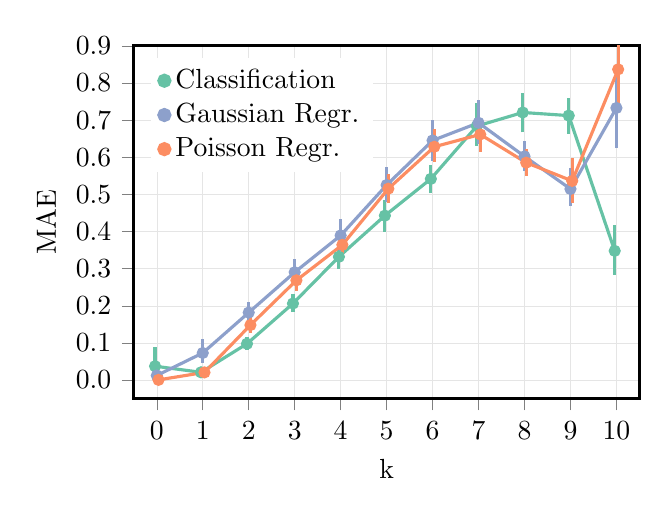
\begin{tikzpicture}

\definecolor{color0}{rgb}{0.917647058823529,0.917647058823529,0.949019607843137}
\definecolor{color1}{RGB}{102,194,165}
\definecolor{color3}{RGB}{252,141,98}
\definecolor{color2}{RGB}{141,160,203}

\begin{axis}[
xlabel={k},
ylabel={MAE},
width=0.66\textwidth,
height=0.5\textwidth,
xmin=-0.5, xmax=10.5,
ymin=-0.05, ymax=0.9,
ytick={-0.1,0,0.1,0.2,0.3,0.4,0.5,0.6,0.7,0.8,0.9},
yticklabels={0.0,0.0,0.1,0.2,0.3,0.4,0.5,0.6,0.7,0.8,0.9},
xtick distance=1,
tick align=outside,
tick pos=left,
ymajorgrids,
xmajorgrids,
axis line style={black},
grid style={line width=.1pt, draw=gray!20},
major grid style={line width=.2pt,draw=gray!20},
legend style={at={(0.03,0.97)}, anchor=north west, draw=none, fill==gray!0},
legend entries={{Classification},{Gaussian Regr.},{Poisson Regr.}},
legend cell align={left}
]
\addplot [only marks, draw=color1, fill=color1, colormap/blackwhite]
table{%
x                      y
-3.750000000000001e-02 +3.735042735042735e-02
+9.625000000000000e-01 +2.086880593756822e-02
+1.962500000000000e+00 +9.780361757105942e-02
+2.962500000000000e+00 +2.061248527679623e-01
+3.962500000000000e+00 +3.319121447028424e-01
+4.962500000000000e+00 +4.427415921668795e-01
+5.962500000000000e+00 +5.417355371900826e-01
+6.962500000000000e+00 +6.838345864661655e-01
+7.962500000000000e+00 +7.204724409448819e-01
+8.962500000000000e+00 +7.120987654320987e-01
+9.962500000000000e+00 +3.478956228956228e-01
};
\addplot [line width=2.00pt, color1, forget plot]
table {%
-0.0375 0.0373504273504274
0.9625 0.0208688059375682
1.9625 0.0978036175710594
2.9625 0.206124852767962
3.9625 0.331912144702842
4.9625 0.44274159216688
5.9625 0.541735537190083
6.9625 0.683834586466165
7.9625 0.720472440944882
8.9625 0.712098765432099
9.9625 0.347895622895623
};
\addplot [line width=2.00pt, color1, forget plot]
table {%
-0.0375 0.00153739316239316
-0.0375 0.0895363247863248
};
\addplot [line width=2.00pt, color1, forget plot]
table {%
0.9625 0.0127919668194717
0.9625 0.0316961362148003
};
\addplot [line width=2.00pt, color1, forget plot]
table {%
1.9625 0.0817797157622739
1.9625 0.114736218776916
};
\addplot [line width=2.00pt, color1, forget plot]
table {%
2.9625 0.182602080879466
2.9625 0.231887514723204
};
\addplot [line width=2.00pt, color1, forget plot]
table {%
3.9625 0.29969315245478
3.9625 0.365779500430663
};
\addplot [line width=2.00pt, color1, forget plot]
table {%
4.9625 0.399341209025117
4.9625 0.485740740740741
};
\addplot [line width=2.00pt, color1, forget plot]
table {%
5.9625 0.502793847566575
5.9625 0.579757805325987
};
\addplot [line width=2.00pt, color1, forget plot]
table {%
6.9625 0.631313700918964
6.9625 0.745908521303258
};
\addplot [line width=2.00pt, color1, forget plot]
table {%
7.9625 0.66682195975503
7.9625 0.773801399825022
};
\addplot [line width=2.00pt, color1, forget plot]
table {%
8.9625 0.663826038159372
8.9625 0.758792368125701
};
\addplot [line width=2.00pt, color1, forget plot]
table {%
9.9625 0.283256523569024
9.9625 0.418800505050505
};
\addplot [only marks, draw=color2, fill=color2, colormap/blackwhite]
table{%
x                      y
+0.000000000000000e+00 +1.235042760510825e-02
+1.000000000000000e+00 +7.290984498750833e-02
+2.000000000000000e+00 +1.817398789856169e-01
+3.000000000000000e+00 +2.903023165133264e-01
+4.000000000000000e+00 +3.893195516533322e-01
+5.000000000000000e+00 +5.250319321950276e-01
+6.000000000000000e+00 +6.450872368282742e-01
+7.000000000000000e+00 +6.927318334579468e-01
+8.000000000000000e+00 +6.023184604114956e-01
+9.000000000000000e+00 +5.145679036776225e-01
+1.000000000000000e+01 +7.327020216319297e-01
};
\addplot [line width=2.00pt, color2, forget plot]
table {%
0 0.0123504276051083
1 0.0729098449875083
2 0.181739878985617
3 0.290302316513326
4 0.389319551653332
5 0.525031932195028
6 0.645087236828274
7 0.692731833457947
8 0.602318460411496
9 0.514567903677623
10 0.73270202163193
};
\addplot [line width=2.00pt, color2, forget plot]
table {%
0 0.00534081213764795
0 0.0241025645566535
};
\addplot [line width=2.00pt, color2, forget plot]
table {%
1 0.0466262830175563
1 0.110413665477342
};
\addplot [line width=2.00pt, color2, forget plot]
table {%
2 0.155333763578286
2 0.211202626282142
};
\addplot [line width=2.00pt, color2, forget plot]
table {%
3 0.257034745460583
3 0.324860619132717
};
\addplot [line width=2.00pt, color2, forget plot]
table {%
4 0.34692829568353
4 0.432953272768193
};
\addplot [line width=2.00pt, color2, forget plot]
table {%
5 0.478991059346331
5 0.574425296684106
};
\addplot [line width=2.00pt, color2, forget plot]
table {%
6 0.590747243298425
6 0.699374426702658
};
\addplot [line width=2.00pt, color2, forget plot]
table {%
7 0.634959278139803
7 0.754830837696791
};
\addplot [line width=2.00pt, color2, forget plot]
table {%
8 0.562505469305648
8 0.6433584856987
};
\addplot [line width=2.00pt, color2, forget plot]
table {%
9 0.468725030223529
9 0.570103260063463
};
\addplot [line width=2.00pt, color2, forget plot]
table {%
10 0.624493893070353
10 0.840917507157558
};
% \path [draw=white, fill opacity=0] (axis cs:0,-0.0600185928210457)
% --(axis cs:0,1.00006922752411);
%
% \path [draw=white, fill opacity=0] (axis cs:1,-0.0600185928210457)
% --(axis cs:1,1.00006922752411);
%
% \path [draw=white, fill opacity=0] (axis cs:-0.5,0)
% --(axis cs:10.5,0);
%
% \path [draw=white, fill opacity=0] (axis cs:-0.5,1)
% --(axis cs:10.5,1);

\addplot [only marks, draw=color3, fill=color3, colormap/blackwhite]
table{%
x                      y
+3.750000000000001e-02 +5.128205128205128e-04
+1.037500000000000e+00 +2.060685439860293e-02
+2.037500000000000e+00 +1.480620155038760e-01
+3.037500000000000e+00 +2.685119748723989e-01
+4.037500000000000e+00 +3.640826873385014e-01
+5.037500000000000e+00 +5.153256704980842e-01
+6.037500000000000e+00 +6.281450872359963e-01
+7.037500000000000e+00 +6.613617376775270e-01
+8.037500000000000e+00 +5.853455818022747e-01
+9.037500000000000e+00 +5.362514029180696e-01
+1.003750000000000e+01 +8.365740740740741e-01
};
\addplot [line width=2.00pt, color3, forget plot]
table {%
0.0375 0.000512820512820513
1.0375 0.0206068543986029
2.0375 0.148062015503876
3.0375 0.268511974872399
4.0375 0.364082687338501
5.0375 0.515325670498084
6.0375 0.628145087235996
7.0375 0.661361737677527
8.0375 0.585345581802275
9.0375 0.53625140291807
10.0375 0.836574074074074
};
\addplot [line width=2.00pt, color3, forget plot]
table {%
0.0375 0.000170940170940171
0.0375 0.000982905982905983
};
\addplot [line width=2.00pt, color3, forget plot]
table {%
1.0375 0.0122647893473041
1.0375 0.0345797860729098
};
\addplot [line width=2.00pt, color3, forget plot]
table {%
2.0375 0.12656976744186
2.0375 0.169559646856158
};
\addplot [line width=2.00pt, color3, forget plot]
table {%
3.0375 0.240591872791519
3.0375 0.298862387122104
};
\addplot [line width=2.00pt, color3, forget plot]
table {%
4.0375 0.332558139534884
4.0375 0.39405684754522
};
\addplot [line width=2.00pt, color3, forget plot]
table {%
5.0375 0.476749680715198
5.0375 0.554259259259259
};
\addplot [line width=2.00pt, color3, forget plot]
table {%
6.0375 0.587143021120294
6.0375 0.676090449954086
};
\addplot [line width=2.00pt, color3, forget plot]
table {%
7.0375 0.614816207184628
7.0375 0.704314954051796
};
\addplot [line width=2.00pt, color3, forget plot]
table {%
8.0375 0.549119641294838
8.0375 0.623103674540682
};
\addplot [line width=2.00pt, color3, forget plot]
table {%
9.0375 0.475597081930415
9.0375 0.597627384960718
};
\addplot [line width=2.00pt, color3, forget plot]
table {%
10.0375 0.727001262626263
10.0375 0.951883417508417
};
\end{axis}

\end{tikzpicture}

%       \end{adjustbox}
%       \caption{by output distribution.}%
%       \label{fig:ssec:exp_fixed_gains/B}
%   \end{subfigure}\hfill%
%   \begin{subfigure}[b]{0.30\textwidth}
%       \centering
%       \begin{adjustbox}{width=\textwidth}
%         % This file was created by matplotlib2tikz v0.6.13.
\begin{tikzpicture}

\definecolor{color0}{rgb}{0.917647058823529,0.917647058823529,0.949019607843137}

\begin{axis}[
xlabel={k},
ylabel={MAE},
width=0.66\textwidth,
height=0.5\textwidth,
xmin=-0.5, xmax=10.5,
ymin=-0.05, ymax=0.9,
ytick={-0.1,0,0.1,0.2,0.3,0.4,0.5,0.6,0.7,0.8,0.9},
yticklabels={0.0,0.0,0.1,0.2,0.3,0.4,0.5,0.6,0.7,0.8,0.9},
xtick distance=1,
tick align=outside,
tick pos=left,
ymajorgrids,
xmajorgrids,
axis line style={black},
grid style={line width=.1pt, draw=gray!20},
major grid style={line width=.2pt,draw=gray!20},
legend entries={{F-CNN},{CNN},{F-CRNN},{CRNN},{RNN~\cite{stoeter17}}},
legend style={at={(0.03,0.97)}, anchor=north west, draw=none, fill=gray!0, font=\scriptsize},
legend cell align={left}
]
\addplot [only marks, draw=FCNN, fill=FCNN, colormap/blackwhite]
table{%
x                      y
-6.250000000000000e-02 +1.609686645533242e-02
+9.375000000000000e-01 +6.810740004287860e-02
+1.937500000000000e+00 +1.871231682694852e-01
+2.937500000000000e+00 +2.900143965558066e-01
+3.937500000000000e+00 +4.082687340469289e-01
+4.937500000000000e+00 +5.654179110829165e-01
+5.937500000000000e+00 +6.553412880013030e-01
+6.937500000000000e+00 +7.385129500517637e-01
+7.937500000000000e+00 +6.676144655364774e-01
+8.937500000000000e+00 +6.725028088197162e-01
+9.937500000000000e+00 +8.343855208151804e-01
};
\addplot [line width=2.00pt, FCNN, forget plot]
table {%
-0.0625 0.0160968664553324
0.9375 0.0681074000428786
1.9375 0.187123168269485
2.9375 0.290014396555807
3.9375 0.408268734046929
4.9375 0.565417911082917
5.9375 0.655341288001303
6.9375 0.738512950051764
7.9375 0.667614465536477
8.9375 0.672502808819716
9.9375 0.83438552081518
};
\addplot [line width=2.00pt, FCNN, forget plot]
table {%
-0.0625 0.00427350433559245
-0.0625 0.032419872278337
};
\addplot [line width=2.00pt, FCNN, forget plot]
table {%
0.9375 0.0406734335280436
0.9375 0.10157898504591
};
\addplot [line width=2.00pt, FCNN, forget plot]
table {%
1.9375 0.149366565919747
1.9375 0.233137736180939
};
\addplot [line width=2.00pt, FCNN, forget plot]
table {%
2.9375 0.254217380758762
2.9375 0.327314815066483
};
\addplot [line width=2.00pt, FCNN, forget plot]
table {%
3.9375 0.374671620453119
3.9375 0.445592879322353
};
\addplot [line width=2.00pt, FCNN, forget plot]
table {%
4.9375 0.520718039641279
4.9375 0.61367780890385
};
\addplot [line width=2.00pt, FCNN, forget plot]
table {%
5.9375 0.600531829466213
5.9375 0.715734995382986
};
\addplot [line width=2.00pt, FCNN, forget plot]
table {%
6.9375 0.673544972183909
6.9375 0.808347258480503
};
\addplot [line width=2.00pt, FCNN, forget plot]
table {%
7.9375 0.600100245278955
7.9375 0.744099954962643
};
\addplot [line width=2.00pt, FCNN, forget plot]
table {%
8.9375 0.585170224673887
8.9375 0.760961468631839
};
\addplot [line width=2.00pt, FCNN, forget plot]
table {%
9.9375 0.656660354222713
9.9375 1.02770763036244
};
\addplot [only marks, draw=CNN, fill=CNN, colormap/blackwhite]
table{%
x                      y
-3.125000000000000e-02 +1.495726509789201e-03
+9.687500000000000e-01 +1.760896459410368e-02
+1.968750000000000e+00 +1.216623599392619e-01
+2.968750000000000e+00 +2.069100901482539e-01
+3.968750000000000e+00 +2.922049940205702e-01
+4.968750000000000e+00 +4.167730962238836e-01
+5.968750000000000e+00 +5.557086000319903e-01
+6.968750000000000e+00 +5.869534927485414e-01
+7.968750000000000e+00 +5.456401261879356e-01
+8.968750000000000e+00 +5.296670419778263e-01
+9.968750000000000e+00 +6.469556705317513e-01
};
\addplot [line width=2.00pt, CNN, forget plot]
table {%
-0.03125 0.0014957265097892
0.96875 0.0176089645941037
1.96875 0.121662359939262
2.96875 0.206910090148254
3.96875 0.29220499402057
4.96875 0.416773096223884
5.96875 0.55570860003199
6.96875 0.586953492748541
7.96875 0.545640126187936
8.96875 0.529667041977826
9.96875 0.646955670531751
};
\addplot [line width=2.00pt, CNN, forget plot]
table {%
-0.03125 0.000569800578609661
-0.03125 0.00242343307596477
};
\addplot [line width=2.00pt, CNN, forget plot]
table {%
0.96875 0.0108382449495332
0.96875 0.0252510370163853
};
\addplot [line width=2.00pt, CNN, forget plot]
table {%
1.96875 0.0968938411976859
1.96875 0.149162000738605
};
\addplot [line width=2.00pt, CNN, forget plot]
table {%
2.96875 0.172551041119997
2.96875 0.243168432323684
};
\addplot [line width=2.00pt, CNN, forget plot]
table {%
3.96875 0.253718057931103
3.96875 0.335432813824626
};
\addplot [line width=2.00pt, CNN, forget plot]
table {%
4.96875 0.357010075388622
4.96875 0.480567972900403
};
\addplot [line width=2.00pt, CNN, forget plot]
table {%
5.96875 0.49686065282448
5.96875 0.629650670435721
};
\addplot [line width=2.00pt, CNN, forget plot]
table {%
6.96875 0.520739347236638
6.96875 0.652126840199934
};
\addplot [line width=2.00pt, CNN, forget plot]
table {%
7.96875 0.500136699940119
7.96875 0.588074144240187
};
\addplot [line width=2.00pt, CNN, forget plot]
table {%
8.96875 0.475188928860774
8.96875 0.57882903330265
};
\addplot [line width=2.00pt, CNN, forget plot]
table {%
9.96875 0.499768520983649
9.96875 0.791559695281866
};
\path [draw=white, fill opacity=0] (axis cs:0,-0.0642762651515782)
--(axis cs:0,1.07970686348216);

\path [draw=white, fill opacity=0] (axis cs:1,-0.0642762651515782)
--(axis cs:1,1.07970686348216);

\path [draw=white, fill opacity=0] (axis cs:-0.5,0)
--(axis cs:10.5,0);

\path [draw=white, fill opacity=0] (axis cs:-0.5,1)
--(axis cs:10.5,1);

\addplot [only marks, draw=FCRNN, fill=FCRNN, colormap/blackwhite]
table{%
x                      y
+0.000000000000000e+00 +6.346153848163752e-02
+1.000000000000000e+00 +7.218220163694986e-02
+2.000000000000000e+00 +1.653028996578414e-01
+3.000000000000000e+00 +2.925664174269669e-01
+4.000000000000000e+00 +4.153029006632313e-01
+5.000000000000000e+00 +5.485312881513033e-01
+6.000000000000000e+00 +6.603152773086178e-01
+7.000000000000000e+00 +7.562656681606015e-01
+8.000000000000000e+00 +6.770195411537229e-01
+9.000000000000000e+00 +5.510662176793674e-01
+1.000000000000000e+01 +6.087962971993969e-01
};
\addplot [line width=2.00pt, FCRNN, forget plot]
table {%
0 0.0634615384816375
1 0.0721822016369499
2 0.165302899657841
3 0.292566417426967
4 0.415302900663231
5 0.548531288151303
6 0.660315277308618
7 0.756265668160601
8 0.677019541153723
9 0.551066217679367
10 0.608796297199397
};
\addplot [line width=2.00pt, FCRNN, forget plot]
table {%
0 0.00327457266575969
0 0.152783119675935
};
\addplot [line width=2.00pt, FCRNN, forget plot]
table {%
1 0.0379811538036914
1 0.117306993108207
};
\addplot [line width=2.00pt, FCRNN, forget plot]
table {%
2 0.142825868812946
2 0.189570772423677
};
\addplot [line width=2.00pt, FCRNN, forget plot]
table {%
3 0.26108166456477
3 0.321173601928928
};
\addplot [line width=2.00pt, FCRNN, forget plot]
table {%
4 0.379186404986292
4 0.450771608875335
};
\addplot [line width=2.00pt, FCRNN, forget plot]
table {%
5 0.503400382091471
5 0.592736270459379
};
\addplot [line width=2.00pt, FCRNN, forget plot]
table {%
6 0.610785893782549
6 0.711432509583583
};
\addplot [line width=2.00pt, FCRNN, forget plot]
table {%
7 0.707322127606271
7 0.805423287159302
};
\addplot [line width=2.00pt, FCRNN, forget plot]
table {%
8 0.627726745471189
8 0.733316930837779
};
\addplot [line width=2.00pt, FCRNN, forget plot]
table {%
9 0.488881408392023
9 0.614322857952468
};
\addplot [line width=2.00pt, FCRNN, forget plot]
table {%
10 0.498625141462493
10 0.723000841983307
};
\addplot [only marks, draw=CRNN, fill=CRNN, colormap/blackwhite]
table{%
x                      y
+3.125000000000000e-02 +1.424501451631833e-03
+1.031250000000000e+00 +7.567488835640818e-03
+2.031250000000000e+00 +7.493540085798669e-02
+3.031250000000000e+00 +1.739301140378820e-01
+4.031250000000000e+00 +2.658627627782701e-01
+5.031250000000000e+00 +3.860508020218169e-01
+6.031250000000000e+00 +5.054331182119932e-01
+7.031250000000000e+00 +5.913394604825403e-01
+8.031250000000000e+00 +5.926655008150419e-01
+9.031250000000000e+00 +4.832023948219176e-01
+1.003125000000000e+01 +3.981481475209950e-01
};
\addplot [line width=2.00pt, CRNN, forget plot]
table {%
0.03125 0.00142450145163183
1.03125 0.00756748883564082
2.03125 0.0749354008579867
3.03125 0.173930114037882
4.03125 0.26586276277827
5.03125 0.386050802021817
6.03125 0.505433118211993
7.03125 0.59133946048254
8.03125 0.592665500815042
9.03125 0.483202394821918
10.03125 0.398148147520995
};
\addplot [line width=2.00pt, CRNN, forget plot]
table {%
0.03125 0.0004985754989735
0.03125 0.00270655276526948
};
\addplot [line width=2.00pt, CRNN, forget plot]
table {%
1.03125 0.00203558178730112
1.03125 0.0145546822128031
};
\addplot [line width=2.00pt, CRNN, forget plot]
table {%
2.03125 0.0569157335567367
2.03125 0.0955408415482242
};
\addplot [line width=2.00pt, CRNN, forget plot]
table {%
3.03125 0.146104894003063
3.03125 0.204166667151622
};
\addplot [line width=2.00pt, CRNN, forget plot]
table {%
4.03125 0.23291343713199
4.03125 0.2977354312345
};
\addplot [line width=2.00pt, CRNN, forget plot]
table {%
5.03125 0.348859443451997
5.03125 0.421471903264116
};
\addplot [line width=2.00pt, CRNN, forget plot]
table {%
6.03125 0.457526017299231
6.03125 0.55380509473705
};
\addplot [line width=2.00pt, CRNN, forget plot]
table {%
7.03125 0.533848510757068
7.03125 0.653164161347108
};
\addplot [line width=2.00pt, CRNN, forget plot]
table {%
8.03125 0.543070136671617
8.03125 0.643294327571819
};
\addplot [line width=2.00pt, CRNN, forget plot]
table {%
9.03125 0.423866442182048
9.03125 0.545838009867325
};
\addplot [line width=2.00pt, CRNN, forget plot]
table {%
10.03125 0.310530652987377
10.03125 0.493304572760114
};
\addplot [only marks, draw=RNN, fill=RNN, colormap/blackwhite]
table{%
x                      y
+6.250000000000000e-02 +1.210826215535890e-03
+1.062500000000000e+00 +2.517645376322615e-02
+2.062500000000000e+00 +1.636520247096787e-01
+3.062500000000000e+00 +3.114775554205700e-01
+4.062500000000000e+00 +4.272179146487926e-01
+5.062500000000000e+00 +5.550588939533989e-01
+6.062500000000000e+00 +6.481481518700176e-01
+7.062500000000000e+00 +7.234753578926187e-01
+8.062500000000000e+00 +6.972878382379093e-01
+9.062500000000000e+00 +7.017583234141570e-01
+1.006250000000000e+01 +7.070005616020540e-01
};
\addplot [line width=2.00pt, RNN, forget plot]
table {%
0.0625 0.00121082621553589
1.0625 0.0251764537632262
2.0625 0.163652024709679
3.0625 0.31147755542057
4.0625 0.427217914648793
5.0625 0.555058893953399
6.0625 0.648148151870018
7.0625 0.723475357892619
8.0625 0.697287838237909
9.0625 0.701758323414157
10.0625 0.707000561602054
};
\addplot [line width=2.00pt, RNN, forget plot]
table {%
0.0625 0.000498575503043061
0.0625 0.00206552708364109
};
\addplot [line width=2.00pt, RNN, forget plot]
table {%
1.0625 0.0152059230939088
1.0625 0.0382776697341815
};
\addplot [line width=2.00pt, RNN, forget plot]
table {%
2.0625 0.137376184544189
2.0625 0.190929156405883
};
\addplot [line width=2.00pt, RNN, forget plot]
table {%
3.0625 0.277707434068703
3.0625 0.350161955888962
};
\addplot [line width=2.00pt, RNN, forget plot]
table {%
4.0625 0.388874532062664
4.0625 0.477535531107479
};
\addplot [line width=2.00pt, RNN, forget plot]
table {%
5.0625 0.501489998066643
5.0625 0.623877187503222
};
\addplot [line width=2.00pt, RNN, forget plot]
table {%
6.0625 0.591823541416117
6.0625 0.716944064002884
};
\addplot [line width=2.00pt, RNN, forget plot]
table {%
7.0625 0.666513509922657
7.0625 0.78691347012718
};
\addplot [line width=2.00pt, RNN, forget plot]
table {%
8.0625 0.642745697520484
8.0625 0.764656240344221
};
\addplot [line width=2.00pt, RNN, forget plot]
table {%
9.0625 0.624979422747464
9.0625 0.786464645104532
};
\addplot [line width=2.00pt, RNN, forget plot]
table {%
10.0625 0.566563200983234
10.0625 0.853794893655846
};
\end{axis}

\end{tikzpicture}

%       \end{adjustbox}
%       \caption{by proposed DNN architecture.}%
%       \label{fig:ssec:exp_fixed_gains/C}
%   \end{subfigure}
%   \caption{}%
%   \label{}
%  \end{figure*}

To find the best parameters we performed training and evaluation for different input representations and output distributions (c.f. \cite{stoeter17}) as well as all proposed architectures resulting in 135 models.
On average each model was trained for 25 epochs before early stopping was engaged.
We present the results filtered by the three factors (Architecture, Input and Output) in Figure~\ref{fig:fixed-gain-results}.
One can see that the overall trend of the count error in MAE is similar regardless of the parametrization: all models are able to reliably distinguish between \(k=0\) and \(k=1\), followed by a nearly linear increase in MAE between \(k=\{1, 2\dots7\}\).
For \(k > 7\) it can be seen that the classification type models have learned the maximum of \(k\) across the dataset, hence the prediction error decreases when \(k\) reaches its maximum.
This is because classification based models intrinsically have access to the maximum number of sources determined by the output vector dimensionality.
Furthermore, one can see that all three factors have only little effect on the overall performance of the model, which is especially the case for small \(k\).
As indicated by Figure~\ref{fig:ssec:exp_fixed_gains/A}, choosing linear STFT as input representation generally results in a better performance compared to MEL and even LOGSTFT.
Concerning the output distribution, a similar observation can be made about classification which outperforms Poisson regression and Gaussian regression, as indicated by Figure~\ref{fig:ssec:exp_fixed_gains/B}.
In Figure~\ref{fig:ssec:exp_fixed_gains/C} the performance of our proposed architectures are compared:
while CNN and CRNN are close, both of them perform better than full frequency band F-CNN and F-CRNN models as well as the recurrent based architecture, proposed in~\cite{stoeter17}.
However, it is interesting that, despite its simplicity, the F-CNN and F-CRNN, perform similarly to the Bi-LSTM architecture.
\par
The results are supported by a statistical evaluation based on mixed effect linear model (see Table~\ref{tab:mixedmodel1}) where \(k\) is modeled as a random effect (for further details we refer to~\cite{Mcculloch06}).
For a fair comparison (i.e. reducing the bias towards classification type network) of all models we only evaluate results for \(k = \{1, 2\dots7\}\); however, all networks were trained on \(k = \{0, \dots, 10\}\).
These results indicate that CRNN performs statistically significantly better than the CNN.\@
Concerning the input representation, we can report that using STFT representation outperforms the log-scaled STFT as well as the MEL representation.
Interestingly, we did not find any significant differences between MEL and STFTLOG in MAE performance.
With respect to the output distributions, we can report that Classification outperforms the other two distributions while Poisson regression performs better than Gaussian regression which confirms the findings made in~\cite{stoeter17} based on the RNN model.
Therefore, we select the CRNN classification model with STFT features for subsequent experiments.
\par
Figure~\ref{fig:complexity} gives an indication of the efficiency of each model and the trade-off between performance and complexity in terms of parameters and floating point multiplications.
It can be seen that the CRNN is not only the one that performs best but also has significantly fewer parameters than the CNN model.
In contrast, the F-CRNN model does only have a fraction of the number of parameters of the other models, which makes it the most suitable model for mobile applications.

\begin{table}[t]
\caption{Mixed Effects Linear Model for \(k = \{1, 2\dots7\}\). Model: \(MAE \sim architecture + feature + objective + (1|k)\)}
\begin{center}
\begin{tabular}{lcccc}
\toprule
Factor                    & Coef.  & Std.Err. &   z    & \(P>|z|\) \\
\midrule
Intercept                      &  0.305 &    0.091 &  3.360 &       0.001 \\
architecture = CRNN            & -0.028 &    0.011 & -2.419 &       0.016 \\
architecture = F-CNN           &  0.102 &    0.011 &  8.976 &       0.000 \\
architecture = F-CRNN          &  0.102 &    0.011 &  8.947 &       0.000 \\
architecture = RNN             &  0.094 &    0.011 &  8.240 &       0.000 \\
feature = STFT                 & -0.079 &    0.009 & -8.946 &       0.000 \\
feature = STFTLOG              & -0.001 &    0.009 & -0.117 &       0.907 \\
objective = P-Regression       &  0.040 &    0.009 &  4.555 &       0.000 \\
objective = G-Regression       &  0.067 &    0.009 &  7.651 &       0.000 \\
Random Effect \(k\)            &  0.057 &    0.297 &        &             \\
\bottomrule
\end{tabular}
\end{center}%
\label{tab:mixedmodel1}
\end{table}

% wrap things up here, describe the ouput shape dimensions and the temporal resolution.

% \begin{table}
%   \caption{Proposed CRNN Architecture}%
%   \label{fig:crnndetail}
%   \centering
% \begin{tabular}{llll}
%   \toprule
%   Layername (type)              & Configuration    & Output Shape    & \# Param\\
%   Input                         &                  &  (500, 201, 1)  & 0 \\
%   Convolution                   & $3\times 3$, 64  &  (498, 199, 64) & 640 \\
%   Convolution                   & $3\times 3$, 32  &  (496, 197, 32) & 18464 \\
%   Max Pooling                   & $3\times 3$      &  (165, 65, 32)  & 0 \\
%   Convolution                   & $3\times 3$, 128 &  (163, 63, 128) & 36992 \\
%   Convolution                   & $3\times 3$, 64  &  (161, 61, 64)  & 73792 \\
%   Max Pooling                   & $3\times 3$      &  (53, 20, 64)   & 0 \\
%   Dropout                       & 0.25             &  (53, 20, 64)   & 0 \\
%   Reshape                       &                  &  (53, 1280)     & 0 \\
%   lstm1 (LSTM)                  & 40               &  (53, 40)       & 211360 \\
%   Temporal Pooling              & $2$              &  (26, 40)       & 0 \\
%   Reshape                       &                  &  (1040)         & 0 \\
%   Fully Connected (FC)          &                  &  (11)            & 11451 \\
%   \midrule
%   & & Total nb params & 352,699 \\
%   \bottomrule
%   \end{tabular}
% \end{table}

\begin{figure}[t]
  \centering
    \begin{adjustbox}{width=0.66\columnwidth}
      % ## CNN 1
%
% * 0-10: 0.2745
% * 1-7: 0.2212
% * total_params: 8666987
% * total_ops: 17332746
%
% ### CRNN 2
%
% * 0-10: 0.2672
% * 1-7: 0.2056
% * total_params: 352699
% * total_ops: 691690
%
% ### F-CRNN 3
%
% * 0-10: 0.3926
% * 1-7: 0.3613
% * total_params: 67459
% * total_ops: 121465
%
% ### F-CNN 4
%
% * 0-10: 0.3807
% * 1-7: 0.3342
% * total_params: 282315
% * total_ops: 563945
%
% ### RNN 5
%
% * 0-10: 0.3777
% * 1-7: 0.3294
% * total_params: 314571
% * total_ops: 581305

\begin{tikzpicture}
\begin{axis}[
    xmode=log,
    xlabel={Nb of Floating Point Operations},
    ylabel={MAE},
    xmin=20000,
    xmax=40000000,
    ymajorgrids,
    yminorgrids,
    xmajorgrids,
    xminorgrids,
    minor y tick num=4,
    enlarge x limits={0.01},
    grid style={line width=.1pt, draw=gray!25},
    major grid style={line width=.2pt,draw=gray!25}
]
\addplot[
    scatter,
    only marks,
    scatter src=explicit,
    mark=*, draw=white, fill=white, black!20,
    visualization depends on={10 * log10(\thisrow{w1}/100000) \as\wone},
    scatter/classes={
        1={fill=CNN},
        2={fill=CRNN},
        3={fill=FCRNN},
        4={fill=FCNN},
        5={fill=RNN}
    },
    scatter/@pre marker code/.append style={
        /tikz/mark size=\wone
    }
]
table[x=x,y=y,meta=w2]{Chapters/08_Analysis_CountNet/figures/complexity.dat};
\addplot[mark=*, fill=white, mark options={draw=white, mark size=0.5pt}] coordinates {(17332746, 0.2212)} node[pin={150, pin edge={thick}}:{CNN (8.66M)}]{};
\addplot[mark=*, fill=white, mark options={draw=white, mark size=0.5pt}] coordinates {(691690, 0.2056)} node[pin={150, pin edge={thick}}:{CRNN (0.45M)}]{};
\addplot[mark=*, fill=white, mark options={draw=white, mark size=0.5pt}] coordinates {(121465, 0.3613)} node[pin={-90, pin edge={thick}}:{F-CRNN (67K)}]{};
\addplot[mark=*, fill=white, mark options={draw=white, mark size=0.5pt}] coordinates {(563945, 0.3342)} node[pin={30, pin edge={thick}}:{F-CNN (0.28M)}]{};
\addplot[mark=*, fill=white, mark options={draw=white, mark size=0.5pt}] coordinates {(581305, 0.3294)} node[pin={-30, pin edge={thick}}:{RNN~\cite{stoeter17} (0.31M)}]{};
\end{axis}
\end{tikzpicture}

    \end{adjustbox}
    \caption{Complexity in number of floating point multiplications and number of weight parameters (in brackets) over performance in MAE of our five proposed models.}%
  \label{fig:complexity}
 \end{figure}

 %!TEX root = ../stoeter_sourcecount.tex
 \section{Evaluation Results}%
 \label{sec:evaluation}
 In this section, we perform several experiments on the proposed CRNN model that has been selected in the previous section.
 We assess the performance of this model by showing the results of three experiments that augment the test data by
 choosing a different dataset, varying amplitude gain levels and introduce reverberation.
 These results also include several baseline methods.
 Furthermore, we present the effect of training sample duration and compare the results from the DNN to human performance gathered in a listening experiment.

 \subsection{Baselines}%
 \label{ssec:baselines}
 In order to make a meaningful comparison to the CRNN model we propose several baseline methods.
 Since we are dealing with a novel task description, related speaker count estimation techniques like those introduced in Section~\ref{sec:introduction}, can hardly be used as baselines.
 Specifically,~\cite{xu13} would not work on fully overlapped speech,~\cite{andrei15_interspeech} does not scale to the size of our dataset, since it requires to cross-correlate the full database against another.
 Finally,~\cite{sayoud10} proposes a feature but does not employ a fully automated system that can be used in a data-driven context.
 We, therefore, decided to propose our own baseline methods.

 \paragraph*{\textbf{VQ}}
 This method uses a feature proposed by Sayoud~\cite{sayoud10} based on 7th MEL filter coefficient (\(\mbox{MFCC}_7\)) which was shown to encode sufficiently important speaker-related information.
 The temporal dimension of \(X\) is squashed down by subtracting the mean and standard deviation as \(X = \overline{\mbox{MFCC}_7} - STD(\mbox{MFCC}_7) \in \mathbb{R}^{1}\).
 In~\cite{sayoud10} the mapping from \(X \Rightarrow \cardinality \) is done by manually thresholding \(X\).
 To translate this into a data-driven approach, we employed a vector quantizer (using k-means) to get an optimal mapping with respect to the sum of squares criterion.
 Further, as preprocessing, we added the same normalization as for our proposed CRNN which in turn decreases the performance of the method significantly as it is highly gain dependent.

 \paragraph*{\textbf{SVM, SVR}}
 We found that the information encoded in the 7th \(\mbox{MFCC}\) coefficient as used in the \textbf{VQ} baseline, may not be sufficient enough to  explain the high variability in our dataset.
 This is especially important for larger speaker counts.
 We therefore extended \textsc{VQ} by including all 20 MFCCs but using the same temporal dimensionality reduction, resulting in \(X = \overline{MFCC} - STD(MFCC) \in \mathbb{R}^{20}\).
 To deal with significantly increased dimensionality of \(X\), we used a support vector machine (SVM) with a radial basis function (RBF) kernel.
 Similarly to our proposed DNN based methods, we treat the output as either a classification problem or a regression problem through the use of support vector regression (SVR).

 \subsection{Results on Gain Variations}%
 \label{ssec:exp_random_gains}
 % * Pick: STFT, Classification
 % * 0db =1.0 gain randomly varied between 0.5 and 2.0
 % * Performance drops slightly
 %
 % * --> CNN and CRNN, are most robust to gain variation
 \begin{table*}[h]
 \tiny

 \caption{Averaged MAE results of different methods on several datasets for \( k = [0 \ldots 10] \) with equal power and random gains (up to $\pm 6~\mbox{dB}$)) as well as reverberation. Bold face indicates the best-performing method.}
 \begin{center}
 \begin{tabular}{lcccccccc}
 \toprule
 Trained on & \multicolumn{7}{c}{\emph{LIBRI}} & \multicolumn{1}{c}{\emph{LIBRI-Reverb}} \\
 \cmidrule(r){2-8} \cmidrule(r){9-9}
 Test Set & \multicolumn{3}{c}{LIBRI} & \multicolumn{2}{c}{THCS10} & \multicolumn{2}{c}{TIMIT} & \multicolumn{1}{c}{LIBRI-Reverb} \\
 \cmidrule(r){2-4} \cmidrule(r){5-6} \cmidrule(r){7-8} \cmidrule(r){9-9}
 Variation &     – &     $\pm 6~\mbox{dB}$ & Reverb &  – &     $\pm 6~\mbox{dB}$ &     – &  $\pm 6~dB$ & Reverb \\
 \midrule
 CRNN    &  $\mathbf{0.27 \pm{0.22}}$ & $\mathbf{0.43 \pm{0.39}}$ & $1.63 \pm{0.22}$ & $\mathbf{0.36 \pm{0.25}}$  & $\mathbf{0.50 \pm{0.46}}$ & $\mathbf{0.31 \pm{0.33}}$ & $\mathbf{0.52 \pm{0.52}}$  &  $\mathbf{0.48 \pm{0.22}}$\\
 RNN~\cite{stoeter17} & $0.38 \pm{0.28}$ & $0.57 \pm{0.49}$ & $1.41 \pm{0.87}$ & $0.58 \pm{0.50}$ &$0.76 \pm{0.72}$ & $0.48 \pm{0.41}$ & $0.72 \pm{0.65}$ & $0.59 \pm{0.43}$\\
 SVR     &  $0.58 \pm{0.27}$ & $0.61 \pm{0.31}$ & $\mathbf{0.76 \pm{0.35}}$ & $0.69 \pm{0.28}$ &  $0.73 \pm{0.32}$ & $0.70 \pm{0.45}$ & $0.62 \pm{0.36}$ & $0.71 \pm{0.35}$ \\
 SVC     &  $0.63 \pm{0.39}$ & $0.66 \pm{0.37}$ & $0.85 \pm{0.51}$ & $0.77 \pm{0.37}$ &  $0.77 \pm{0.36}$ & $0.89 \pm{0.75}$ & $0.76 \pm{0.61}$ & $0.78 \pm{0.45}$ \\
 VQ \cite{sayoud10} &  $2.41 \pm{1.08}$ & $2.41 \pm{1.06}$ & $2.41 \pm{1.08}$ & $2.98 \pm{1.62}$ &  $2.98 \pm{1.60}$ & $2.13 \pm{1.06}$ & $2.15 \pm{1.07}$ & $2.41 \pm{1.13}$ \\
 MEAN    &  $2.73 \pm{1.63}$ & $2.73 \pm{1.63}$ & $2.73 \pm{1.63}$ & $2.73 \pm{1.64}$ &  $2.73 \pm{1.63}$ & $2.73 \pm{1.63}$ & $2.73 \pm{1.63}$ & $2.73 \pm{1.63}$ \\
 \bottomrule
 \end{tabular}
 \end{center}
 \label{tab:expgainreverb}
 \end{table*}
 In our parameter optimization in Section~\ref{sec:hyperparameters} we evaluated  mixtures with speakers having equal power.
 In a more realistic scenario, speakers often differ in volume between utterances.
 We simulate this by introducing gain factors between 0.5 and 2.0, randomly applied to the sources, hence resulting in a deviation of $6~dB$ compared to the reference where all speakers are mixed to have equal power.
 We applied this variation only to the test data to evaluate how models generalize to this updated condition.
 The results of this experiment are presented in Table~\ref{tab:expgainreverb}.
 \textbf{MEAN} corresponds to the case when \(\cardinality = 5\) is predicted for all test samples.
 Our results indicate that augmenting the mixture gains does have an impact on performance, for both, our proposed CRNN model as well as the baseline methods.
 E.g.\ for the CRNN model the performance drops by 60\% from 0.27 MAE to 0.43 MAE on the \emph{LIBRI Speech} test set, which is still about 40\% better than the second best-performing method \emph{SVR} which drops from 0.58 MAE to 0.61 MAE.\@

 \subsection{Results on Different Datasets}%
 \label{ssec:r_datasets}
 We also present results on two additional datasets.
 Again, we only changed the test data; all networks were trained on \emph{LIBRI Speech}.
 Compared to \emph{LIBRI Speech}, the \emph{TIMIT} database has an overall lower recording quality.
 This is reflected by our results where the performance in MAE drops only slightly between these two datasets.
 Interestingly, even when we look at the results of the Mandarin language \emph{THCS10} dataset, performance drops only slightly.
 More precisely, for our proposed CRNN model, test performance on \emph{THCS10} is even better than on its own \emph{LIBRI} dataset with gain variations.
 These results suggest that the trained model is speaker and language independent.

 % * Pick best: CRNN, STFT, Classification
 % * TIMIT (slight drop)
 % * German Dataset (medium drop)
 % * THCS Chinese (large drop)

 \subsection{Effect of Reverberant Signals}%
 \label{ssec:exp_reverb}
 % * Pick best: CRNN, STFT, Classification
 % * Generated simulated using @hab RIR Generator
 % * test room: [3.5, 4.5, 2.5]
 % * receiver position at [1, 1, 1]
 % * generating 350 RIRs for each room: between 100ms and 500ms
 % * generating 10 unique source positions for each room: min distance 0.1 to walls
 % * --> Significant Performance Drop (diff 2.0 MAE)
 % * Retrained using train room: [3, 4, 2] and valid room: [4, 5, 3]
 % * Performance back to (0.6 MAE)
 Different acoustical conditions such as increased reverberation time were shown~\cite{Pasha17_reverb} to have a large effect in speaker counting.
 To analyze this effect, different acoustic conditions were simulated by generating the room impulse responses using the image method~\cite{Allen79, Habets16}.
 For this experiment we set up an acoustical room with dimension ($3.5~\mbox{m} \times 4.5~\mbox{m} \times 2.5~\mbox{m}$)
 The microphone was positioned at (1m, 1m, 1m).
 For the mentioned room, 350 different reverberation times were selected uniformly sampled between 0.1 and 0.5 seconds.
 For each of these reverberation times, we generated unique room impulse responses that correspond to individual source positions which have minimum distance $0.1~\mbox{m}$ to the walls and are otherwise positioned randomly on the (X, Y, 1m) plane.
 Each speaker's signal was convolved with a randomly selected room impulse response before mixing.
 Results, again, are shown in Table~\ref{tab:expgainreverb}.
 For the first time, we can see that the CRNN model significantly drops in performance from 0.27 MAE to 1.64 MAE, whereas the SVR and SVM baselines are only affected slightly.
 This is expected as these baselines are using a temporal aggregation of all frames, whereas the CRNN is based on smaller (\(3 \times 3\)) convolutional filter operations that are able to capture the room acoustics as well.
 If we assume that our trained deep learning model is fully speaker independent, a mixture of two utterances from the same speaker would get the same count estimate as two different speakers.
 Hence, reverberation tends to result in overestimation and we observed this even for \(k = 1\) where it, in turn, resulted in an increase in MAE.
 \par
 To further investigate whether the overestimation can be reduced via training with reverberant samples, we created a separate set of room impulse responses for the training dataset with different room dimensions so that the model cannot learn the acoustical conditions from the training dataset.
 From the results shown in the last column of Table~\ref{tab:expgainreverb} we can see that the retrained CRNN is able to outperform the baselines again.
 Therefore, when retrained with reverberant samples, the proposed model is able to better discriminate between a reverberant component of the same speaker and contributions from different speakers.
 For robustness against different acoustic conditions, it is essential to include reverberant samples in the training dataset.

 \subsection{Effect of Duration and Overlap Detection Error}%
 \label{ssec:exp_duration}
 % * Pick best: CRNN, STFT, Classification
 % * (Re) Trained and evaluated on (1s...9s)
 % * Longer context
 % * Shorter context
 In our last experiment we want to address the influence of the input duration length \(D\).
 In a real-world application this parameter would be chosen as small as a possible, because a longer input duration adds both algorithmic and computational delay to a real-time system.
 In a small experiment, we took the proposed CRNN and retrained it using a different number of input frames ranging from 100 to 900 frames (corresponding to one to nine seconds of audio).
 For each input duration, we trained the CRNN with three different initial seeds.
 Results are shown in Figure~\ref{fig:timesteps}.
 It can be seen that five second duration is a good trade-off between performance and delay.
 If latency is critical, keeping \(D\) above 2 seconds is recommended for good results.
 For segments as short as 1 second the MAE of around 0.6 is almost twice as high as for segments of 5 seconds duration.
 However, if instead of the count estimation MAE we compute the accuracy to detect overlap \(k > 1\) vs.\ non-overlap \(k \in {0, 1}\), we still achieve 98.7\% accuracy (precision: 99.7\%, recall: 98.7\%). This shows that our system can be effectively used to address overlap detection.

 \begin{figure}[h!]
     \centering
     \centering
     \begin{adjustbox}{width=0.8\columnwidth}
       % This file was created by matplotlib2tikz v0.6.13.
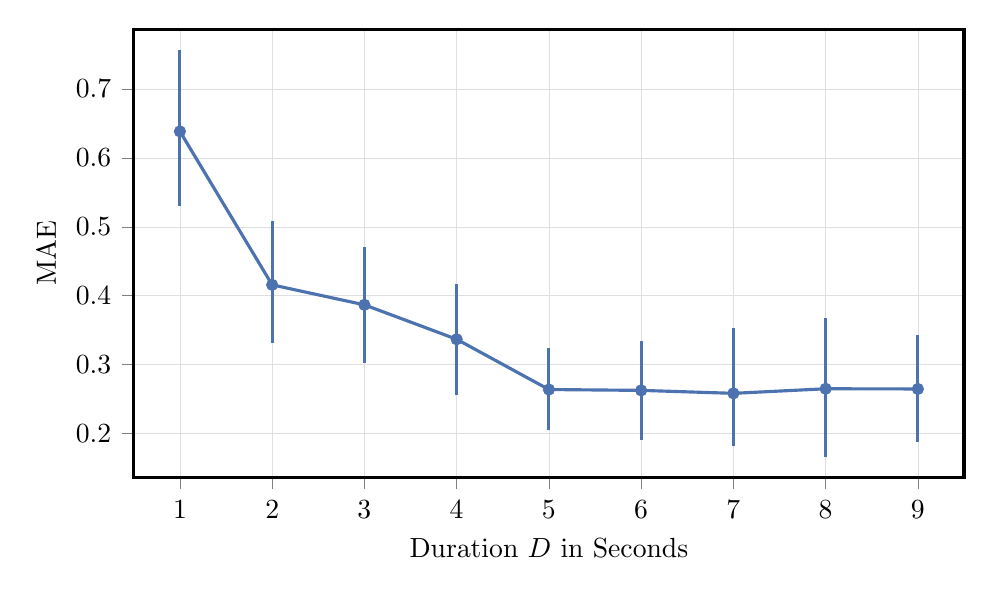
\begin{tikzpicture}

\definecolor{color1}{rgb}{0.298039215686275,0.447058823529412,0.690196078431373}
\definecolor{color0}{rgb}{0.917647058823529,0.917647058823529,0.949019607843137}

\begin{axis}[
xlabel={Duration \(D\) in Seconds},
ylabel={MAE},
xmin=-0.5, xmax=8.5,
ymin=0.135857456148673, ymax=0.786816272987562,
xtick={0,1,2,3,4,5,6,7,8},
xticklabels={1,2,3,4,5,6,7,8,9},
ytick={0.1,0.2,0.3,0.4,0.5,0.6,0.7,0.8},
yticklabels={0.0,0.2,0.3,0.4,0.5,0.6,0.7,},
tick align=outside,
tick pos=left,
xmajorgrids,
ymajorgrids,
width=\columnwidth,
height=0.6\columnwidth,
axis line style={black},
grid style={line width=.1pt, draw=gray!25},
major grid style={line width=.2pt,draw=gray!25},
]
\addplot [only marks, draw=color1, fill=color1, colormap/blackwhite]
table{%
x                      y
+0.000000000000000e+00 +6.385012990646495e-01
+1.000000000000000e+00 +4.156636288682126e-01
+2.000000000000000e+00 +3.866786050449682e-01
+3.000000000000000e+00 +3.366750172732503e-01
+4.000000000000000e+00 +2.637021331951673e-01
+5.000000000000000e+00 +2.624647418728959e-01
+6.000000000000000e+00 +2.581671791258833e-01
+7.000000000000000e+00 +2.647957418016120e-01
+8.000000000000000e+00 +2.645404355185759e-01
};
% \addplot[mark=*, fill=black, mark options={mark size=0.20pt}]
% coordinates {
%   (5, 0.26} node[pin={1, pin edge={thick}}:{Selected Duration}]{};
\addplot [line width=2.00pt, color1, forget plot]
table {%
0 0.638501299064649
1 0.415663628868213
2 0.386678605044968
3 0.33667501727325
4 0.263702133195167
5 0.262464741872896
6 0.258167179125883
7 0.264795741801612
8 0.264540435518576
};
\addplot [line width=2.00pt, color1, forget plot]
table {%
0 0.529501745070873
0 0.757227235858521
};
\addplot [line width=2.00pt, color1, forget plot]
table {%
1 0.331229177698919
1 0.50777318536896
};
\addplot [line width=2.00pt, color1, forget plot]
table {%
2 0.302866441412883
2 0.470527138303221
};
\addplot [line width=2.00pt, color1, forget plot]
table {%
3 0.256214672080081
3 0.416434186077932
};
\addplot [line width=2.00pt, color1, forget plot]
table {%
4 0.205581195002823
4 0.323809986137185
};
\addplot [line width=2.00pt, color1, forget plot]
table {%
5 0.190651073067454
5 0.334762156170043
};
\addplot [line width=2.00pt, color1, forget plot]
table {%
6 0.181574955025837
6 0.352612918248687
};
\addplot [line width=2.00pt, color1, forget plot]
table {%
7 0.165446493277713
7 0.367320912424733
};
\addplot [line width=2.00pt, color1, forget plot]
table {%
8 0.18797697232341
8 0.343365533924186
};
% \path [draw=black, fill opacity=0] (axis cs:500,0.135857456148673)
% --(axis cs:500,0.786816272987562);
%
% \path [draw=white, fill opacity=0] (axis cs:1,0.135857456148673)
% --(axis cs:1,0.786816272987562);
%
% \path [draw=white, fill opacity=0] (axis cs:-0.5,0)
% --(axis cs:8.5,0);
%
% \path [draw=white, fill opacity=0] (axis cs:-0.5,1)
% --(axis cs:8.5,1);

\end{axis}

\end{tikzpicture}

     \end{adjustbox}
     \caption{Evaluation of trained CRNN networks over different input duration length \(D\). Error bars show 95\% confidence intervals.}%
     \label{fig:timesteps}
  \end{figure}

 \vspace*{-0.25cm}%
 \subsection{Listening Experiment}%
 \label{ssec:listening_experiment}
 % * Reference existing listening tests which report the same thing
 % * Are we really doing it? We can decide on this once the first full draft is ready.
To compare the results of our trained CRNN on our synthesized dataset to human performance, we chose to compare the machine model against the experiments made in~\cite{kawashima15, kashino96} and our own as described in Section~TODO.
% The results of our lab-based experiments are shown in Figure~\ref{fig:experiment}.

 % Kawashima et al.\ found in extensive experiments using Japanese speech samples, that participants were able to correctly estimate up to three simultaneously active speakers without using any spatial cues.
 % We conducted our own study using the simulated data from the \emph{LIBRI Speech} (power normalized) set mentioned earlier in Section~\ref{ssec:corpus}.
 % We therefore randomly selected 10 samples for each \(\cardinality \in [0, \ldots, 10]\), resulting in 100 mixtures of 5~seconds duration each.
 % The experiment was done using \emph{between-group design}, where one group (blind experiment) did not get any prior information about the maximum number of speakers in the test set (similar to~\cite{kawashima15}).
 % However, the maximum number of speakers was revealed to the other group (informed experiment), which is more related to our data-driven, classification based CRNN.
 % Further, none of the participants received any feedback about the error made during the trials.
 % Similarly to~\cite{kawashima15}, lab-based experiments were conducted with ten participants for each group (\(n=20\)) using a custom designed web-based software.\footnote{The experiment is made available through the accompanying website.}
 % In all previous experiments, we used the mean absolute error metric which does not reveal over and underestimation errors.
 % We therefore decided to report the average response for each group of \(k\).
 % The results of our lab-based experiments are shown in Figure~\ref{fig:experiment}.
 The results for up to three speakers indicate that humans perform similarly (or better in terms of variance) compared to our proposed CRNN model.
 % Results of the blind experiment show that underestimation becomes apparent for \(k > 3\).
 % As a reference, we also included the average results from~\cite{kawashima15} (Experiment 1, 5~seconds durations) which shows similar results compared to our blind experiment.
 For larger speaker counts, the gap between humans and algorithm is almost three speakers on average.
 Interestingly, the results of the informed experiment reveal that this gap closes down to an average difference of one speaker.
 Finally, we can report that the machine model reached superhuman performance.
 Unlike humans, the CRNN is subject to over-estimations for \(4 < k \leq 9\).
 However, with extensive training, humans might be able to perform on par.
 When we asked participants about the strategy they pursued, many reported that with more than three speakers it is not possible to identify (and count) the speakers but rather compare the \emph{density} of the speech to that of 1-3 speakers.
 For higher speaker counts, participants reported that the integrated phoneme activity was a relevant cue, supporting our previously mentioned hypothesis.

\begin{figure}[t!]
   \centering
   \begin{adjustbox}{width=0.7\columnwidth}
     % This file was created by matplotlib2tikz v0.6.13.
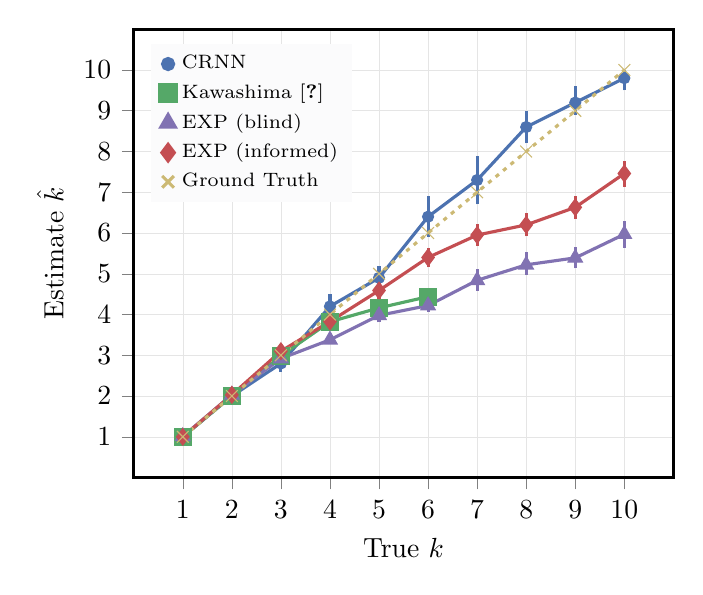
\begin{tikzpicture}

\definecolor{color1}{rgb}{0.298039215686275,0.447058823529412,0.690196078431373}
\definecolor{color0}{rgb}{0.917647058823529,0.917647058823529,0.949019607843137}
\definecolor{color4}{rgb}{0.768627450980392,0.305882352941176,0.32156862745098}
\definecolor{color2}{rgb}{0.333333333333333,0.658823529411765,0.407843137254902}
\definecolor{color5}{rgb}{0.8,0.725490196078431,0.454901960784314}
\definecolor{color3}{rgb}{0.505882352941176,0.447058823529412,0.698039215686274}

\begin{axis}[
xlabel={True \(k\)},
ylabel={Estimate \(\hat{k}\)},
xmin=-1, xmax=10,
ymin=0, ymax=11,
ytick={1,2,3,4,5,6,7,8,9,10},
xtick={0,1,2,3,4,5,6,7,8,9},
xticklabels={1,2,3,4,5,6,7,8,9,10},
tick align=outside,
tick pos=left,
ymajorgrids,
xmajorgrids,
grid style={line width=.1pt, draw=gray!20},
major grid style={line width=.2pt,draw=gray!20},
axis line style={black},
legend style={at={(0.03,0.97)}, anchor=north west, draw=none, fill=color0!20, font=\scriptsize},
legend cell align={left},
legend entries={{CRNN},{Kawashima~\cite{kawashima15}}, {EXP (blind)}, {EXP (informed)},{Ground Truth}}
]
\addplot [only marks, draw=color1, fill=color1, colormap/blackwhite]
table{%
x                      y
+0.000000000000000e+00 +1.000000000000000e+00
+1.000000000000000e+00 +2.000000000000000e+00
+2.000000000000000e+00 +2.800000000000000e+00
+3.000000000000000e+00 +4.200000000000000e+00
+4.000000000000000e+00 +4.900000000000000e+00
+5.000000000000000e+00 +6.400000000000000e+00
+6.000000000000000e+00 +7.300000000000000e+00
+7.000000000000000e+00 +8.600000000000000e+00
+8.000000000000000e+00 +9.199999999999999e+00
+9.000000000000000e+00 +9.800000000000001e+00
};
\addplot [line width=1.5pt, color1, forget plot]
table {%
0 1
1 2
2 2.8
3 4.2
4 4.9
5 6.4
6 7.3
7 8.6
8 9.2
9 9.8
};
\addplot [line width=1.5pt, color1, forget plot]
table {%
0 1
0 1
};
\addplot [line width=1.5pt, color1, forget plot]
table {%
1 2
1 2
};
\addplot [line width=1.5pt, color1, forget plot]
table {%
2 2.5975
2 3
};
\addplot [line width=1.5pt, color1, forget plot]
table {%
3 4
3 4.5
};
\addplot [line width=1.5pt, color1, forget plot]
table {%
4 4.6
4 5.2
};
\addplot [line width=1.5pt, color1, forget plot]
table {%
5 5.9
5 6.9
};
\addplot [line width=1.5pt, color1, forget plot]
table {%
6 6.7
6 7.9
};
\addplot [line width=1.5pt, color1, forget plot]
table {%
7 8.2
7 9
};
\addplot [line width=1.5pt, color1, forget plot]
table {%
8 8.8975
8 9.6
};
\addplot [line width=1.5pt, color1, forget plot]
table {%
9 9.5
9 10
};
\addplot [only marks, mark size=3.0, mark=square*, draw=color2, fill=color2, colormap/blackwhite]
table{%
x                      y
+0.000000000000000e+00 +1.000000000000000e+00
+1.000000000000000e+00 +2.000000000000000e+00
+2.000000000000000e+00 +2.987442378071903e+00
+3.000000000000000e+00 +3.821715111593599e+00
+4.000000000000000e+00 +4.163430371330779e+00
+5.000000000000000e+00 +4.438511376242037e+00
};
\addplot [line width=1.5pt, color2, forget plot]
table {%
0 1
1 2
2 2.9874423780719
3 3.8217151115936
4 4.16343037133078
5 4.43851137624204
6 nan
7 nan
8 nan
9 nan
};
\addplot [line width=1.5pt, color2, forget plot]
table {%
0 nan
0 nan
};
\addplot [line width=1.5pt, color2, forget plot]
table {%
1 nan
1 nan
};
\addplot [line width=1.5pt, color2, forget plot]
table {%
2 nan
2 nan
};
\addplot [line width=1.5pt, color2, forget plot]
table {%
3 nan
3 nan
};
\addplot [line width=1.5pt, color2, forget plot]
table {%
4 nan
4 nan
};
\addplot [line width=1.5pt, color2, forget plot]
table {%
5 nan
5 nan
};
\addplot [line width=1.5pt, color2, forget plot]
table {%
6 nan
6 nan
};
\addplot [line width=1.5pt, color2, forget plot]
table {%
7 nan
7 nan
};
\addplot [line width=1.5pt, color2, forget plot]
table {%
8 nan
8 nan
};
\addplot [line width=1.5pt, color2, forget plot]
table {%
9 nan
9 nan
};

\addplot [only marks, mark size=3.0, mark=triangle*, draw=color3, fill=color3, colormap/blackwhite]
table{%
x                      y
+0.000000000000000e+00 +1.010000000000000e+00
+1.000000000000000e+00 +2.030000000000000e+00
+2.000000000000000e+00 +2.920000000000000e+00
+3.000000000000000e+00 +3.380000000000000e+00
+4.000000000000000e+00 +3.980000000000000e+00
+5.000000000000000e+00 +4.220000000000000e+00
+6.000000000000000e+00 +4.840000000000000e+00
+7.000000000000000e+00 +5.220000000000000e+00
+8.000000000000000e+00 +5.390000000000000e+00
+9.000000000000000e+00 +5.970000000000000e+00
};
\addplot [line width=1.5pt, color3, forget plot]
table {%
0 1.01
1 2.03
2 2.92
3 3.38
4 3.98
5 4.22
6 4.84
7 5.22
8 5.39
9 5.97
};
\addplot [line width=1.5pt, color3, forget plot]
table {%
0 1
0 1.03
};
\addplot [line width=1.5pt, color3, forget plot]
table {%
1 2
1 2.07
};
\addplot [line width=1.5pt, color3, forget plot]
table {%
2 2.78975
2 3.05
};
\addplot [line width=1.5pt, color3, forget plot]
table {%
3 3.27
3 3.5
};
\addplot [line width=1.5pt, color3, forget plot]
table {%
4 3.80975
4 4.16025
};
\addplot [line width=1.5pt, color3, forget plot]
table {%
5 4.06
5 4.4
};
\addplot [line width=1.5pt, color3, forget plot]
table {%
6 4.58
6 5.11
};
\addplot [line width=1.5pt, color3, forget plot]
table {%
7 4.97
7 5.53
};
\addplot [line width=1.5pt, color3, forget plot]
table {%
8 5.13
8 5.66
};
\addplot [line width=1.5pt, color3, forget plot]
table {%
9 5.64
9 6.29
};
\addplot [only marks, mark size=3.0, mark=diamond*, draw=color4, fill=color4, colormap/blackwhite]
table{%
x                      y
+0.000000000000000e+00 +1.000000000000000e+00
+1.000000000000000e+00 +2.030000000000000e+00
+2.000000000000000e+00 +3.100000000000000e+00
+3.000000000000000e+00 +3.830000000000000e+00
+4.000000000000000e+00 +4.590000000000000e+00
+5.000000000000000e+00 +5.400000000000000e+00
+6.000000000000000e+00 +5.950000000000000e+00
+7.000000000000000e+00 +6.200000000000000e+00
+8.000000000000000e+00 +6.630000000000000e+00
+9.000000000000000e+00 +7.460000000000000e+00
};
\addplot [line width=1.5pt, color4, forget plot]
table {%
0 1
1 2.03
2 3.1
3 3.83
4 4.59
5 5.4
6 5.95
7 6.2
8 6.63
9 7.46
};
\addplot [line width=1.5pt, color4, forget plot]
table {%
0 1
0 1
};
\addplot [line width=1.5pt, color4, forget plot]
table {%
1 1.97
1 2.1
};
\addplot [line width=1.5pt, color4, forget plot]
table {%
2 3
2 3.21
};
\addplot [line width=1.5pt, color4, forget plot]
table {%
3 3.67
3 3.98
};
\addplot [line width=1.5pt, color4, forget plot]
table {%
4 4.39
4 4.8
};
\addplot [line width=1.5pt, color4, forget plot]
table {%
5 5.16
5 5.64
};
\addplot [line width=1.5pt, color4, forget plot]
table {%
6 5.69
6 6.23
};
\addplot [line width=1.5pt, color4, forget plot]
table {%
7 5.91975
7 6.48
};
\addplot [line width=1.5pt, color4, forget plot]
table {%
8 6.34
8 6.92
};
\addplot [line width=1.5pt, color4, forget plot]
table {%
9 7.14
9 7.76025
};
\addplot [only marks, mark size=3.0, draw=color5, mark=x, fill=color5, colormap/blackwhite]
table{%
x                      y
+0.000000000000000e+00 +1.000000000000000e+00
+1.000000000000000e+00 +2.000000000000000e+00
+2.000000000000000e+00 +3.000000000000000e+00
+3.000000000000000e+00 +4.000000000000000e+00
+4.000000000000000e+00 +5.000000000000000e+00
+5.000000000000000e+00 +6.000000000000000e+00
+6.000000000000000e+00 +7.000000000000000e+00
+7.000000000000000e+00 +8.000000000000000e+00
+8.000000000000000e+00 +9.000000000000000e+00
+9.000000000000000e+00 +1.000000000000000e+01
};
\addplot [line width=1.5pt, color5, dotted, forget plot]
table {%
0 1
1 2
2 3
3 4
4 5
5 6
6 7
7 8
8 9
9 10
};
\addplot [line width=1.5pt, color5, forget plot]
table {%
0 nan
0 nan
};
\addplot [line width=1.5pt, color5, forget plot]
table {%
1 nan
1 nan
};
\addplot [line width=1.5pt, color5, forget plot]
table {%
2 nan
2 nan
};
\addplot [line width=1.5pt, color5, forget plot]
table {%
3 nan
3 nan
};
\addplot [line width=1.5pt, color5, forget plot]
table {%
4 nan
4 nan
};
\addplot [line width=1.5pt, color5, forget plot]
table {%
5 nan
5 nan
};
\addplot [line width=1.5pt, color5, forget plot]
table {%
6 nan
6 nan
};
\addplot [line width=1.5pt, color5, forget plot]
table {%
7 nan
7 nan
};
\addplot [line width=1.5pt, color5, forget plot]
table {%
8 nan
8 nan
};
\addplot [line width=1.5pt, color5, forget plot]
table {%
9 nan
9 nan
};
\end{axis}

\end{tikzpicture}

   \end{adjustbox}
   \caption{Average responses from humans (\
   {EXP} and \emph{Kawashima}
~\cite{kawashima15}) compared to our proposed CRNN. Error bars show 95\% confidence intervals.}%
   \label{fig:experiment}
\end{figure}

\section{Understanding CountNet}%
\label{sec:ablation}
\begin{figure}[t]
  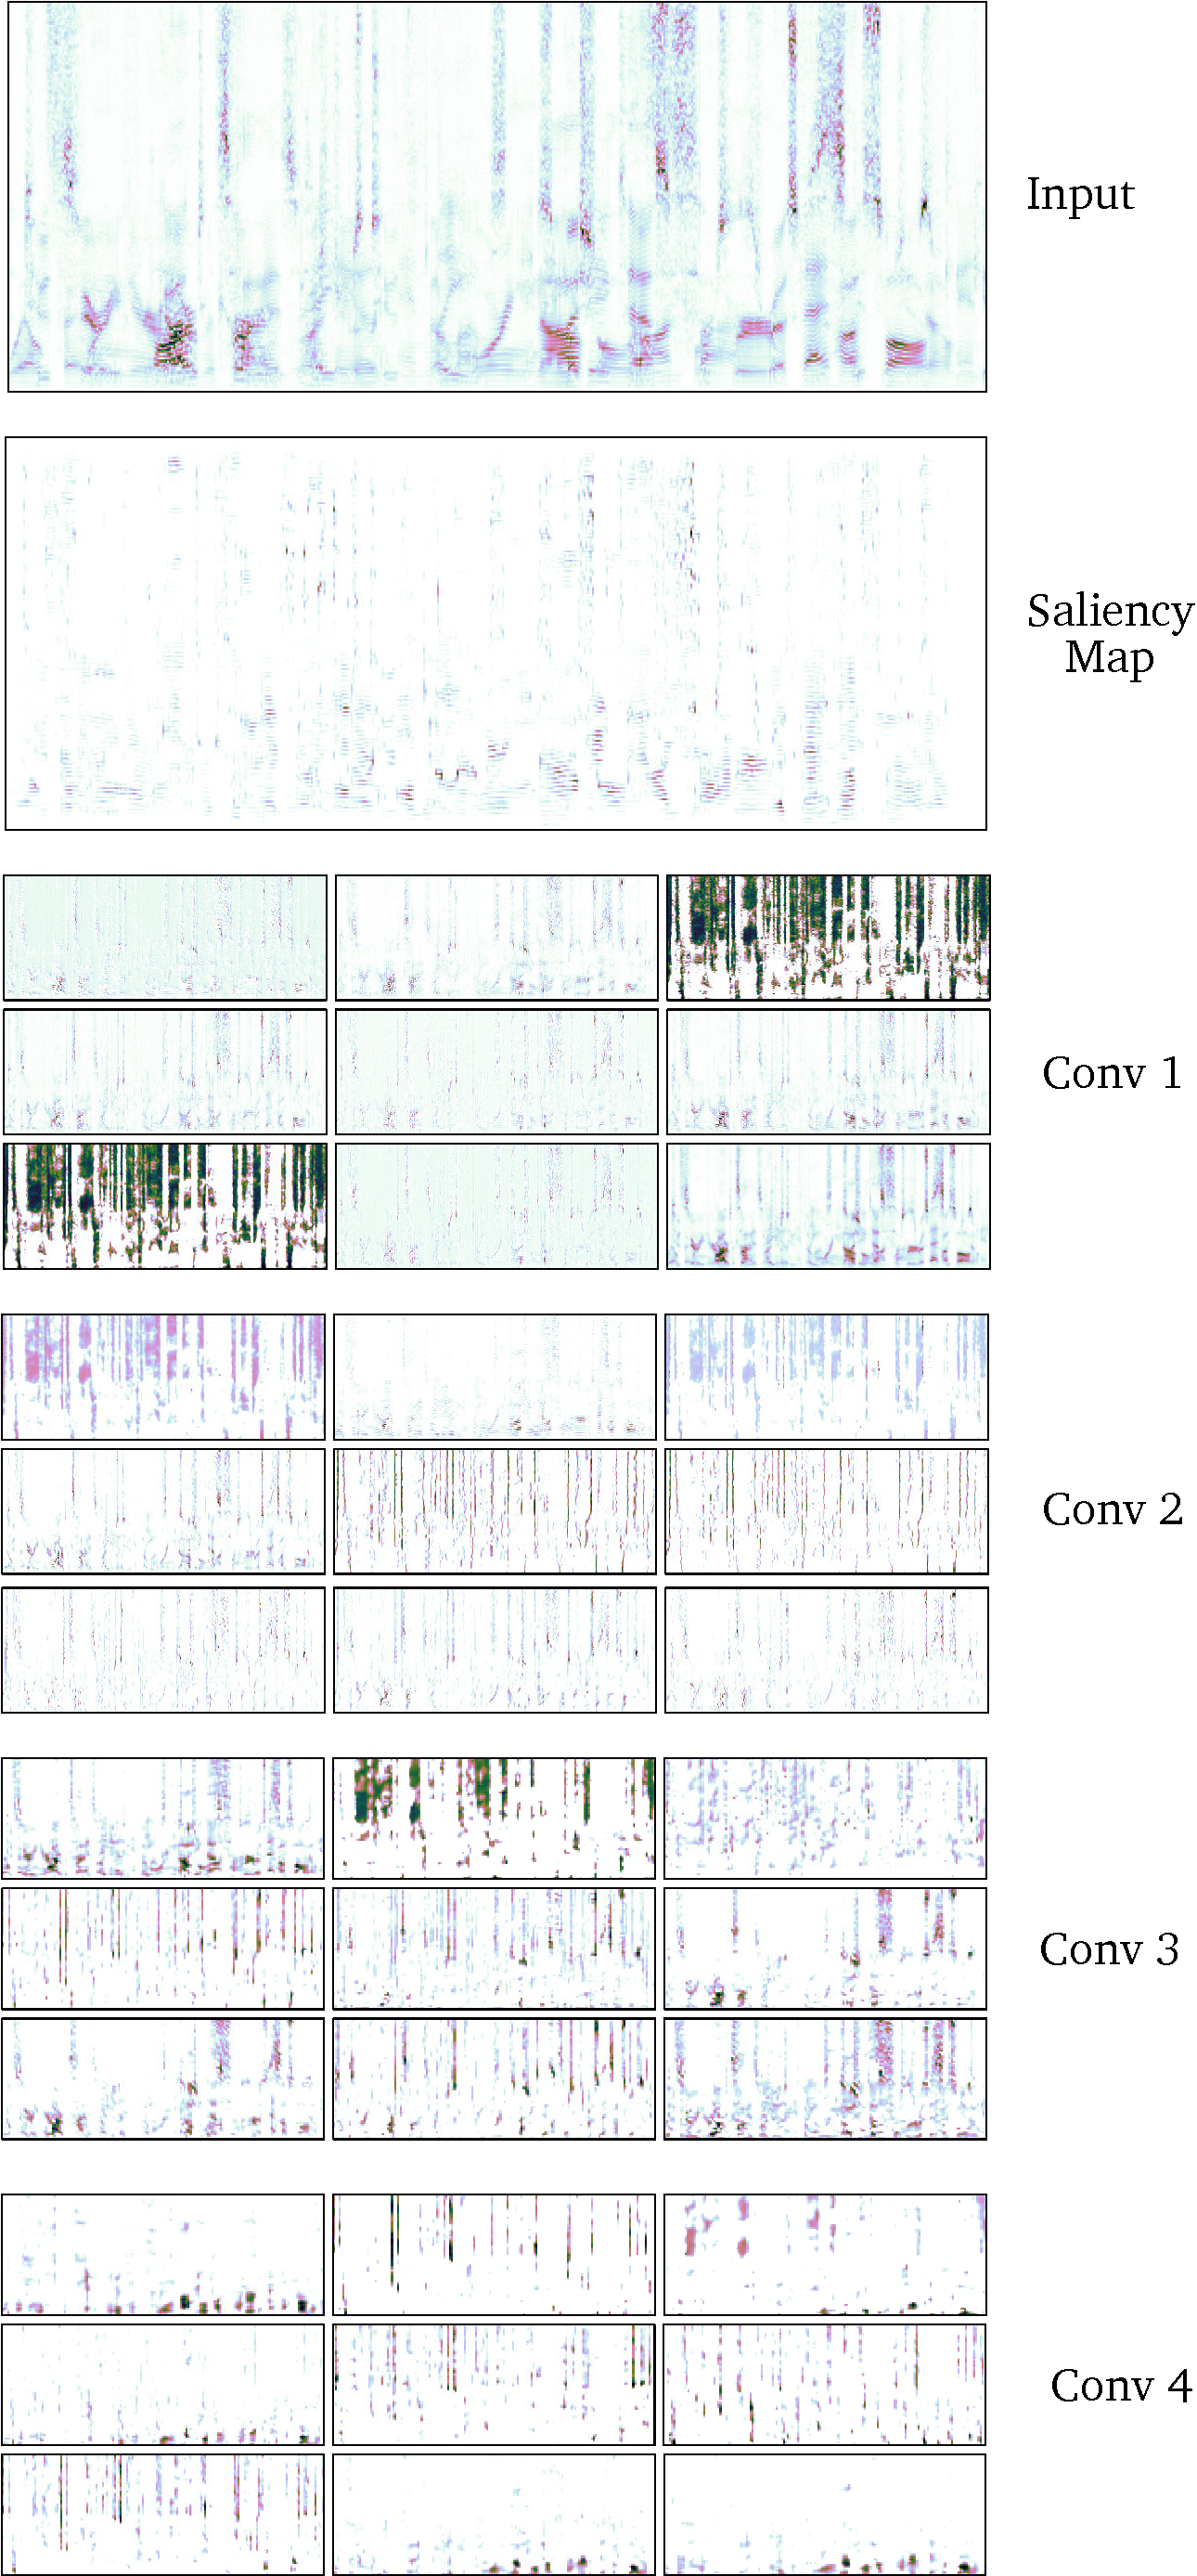
\includegraphics[width=\columnwidth, height=0.65\paperheight, keepaspectratio]{Chapters/08_Analysis_CountNet/figures/outputs.pdf}
  \caption{Illustration of intermediate outputs from the proposed CRNN for each convolutional layer for a given input with \(k=3\) speakers. Saliency map shows positive saliency of guided backpropagation~\cite{Springenberg14}. For each convolutional layer the nine most relevant filters were selected based on their loss with respect to the input.}%
\label{fig:convoutputs}
\end{figure}
% Select best-performing system (CRNN, Classification, STFT) and analyse how it achieves the performance.
In this section, we focus on the problem of interpreting the strategy undergone by this system for successful counting.

\subsection{Saliency Maps}
We first conducted a visual analysis based on salience map representations~\cite{Simonyan13}.
% taken from https://github.com/Lasagne/Recipes/blob/master/examples/Saliency%20Maps%20and%20Guided%20Backpropagation.ipynb
In the deep learning context, saliency maps are visualizations that are able to show which specific input elements a neural network used for a particular prediction. This allows an object classifier to be used for object localization or in the case of audio spectrograms, which time-frequency bins are most relevant.
The common idea is to compute the gradient of the model's prediction with respect to the input, holding the weights fixed. This determines which input elements need to be changed the least to affect the prediction the most.
\par
In this work, we used guided backpropagation, first introduced in~\cite{Springenberg14} and successfully deployed in~\cite{schluter16} to compute a saliency map for singing voice detection.
For a given input of a three-speaker mixture, we depicted the saliency map in Figure~\ref{fig:convoutputs}.
The saliency map indicates that our proposed model does not rely much on the overlapped parts but instead utilize many of the single speaker time-frequency bins as well as many high-frequency components such as plosives and fricative phonemes.\par
While the saliency map confirms that the network does exploit both low and high-frequency content from the input signal, it is not sufficient to conjecture about the strategy implemented in the network.

\subsection{Ablation Analysis}
To provide further insight, we propose another layer-wise analysis, that provides information concerning the behavior of the model at different successive layers.
While we cannot show all filter outputs (e.g. 64, for the first layer), instead, for each filter, we compute its loss with respect to the input of the model using gradient update and sort the filters according to their loss behavior.\par

Figure~\ref{fig:convoutputs} depicts the nine highest loss outputs per convolutional layer.
We can observe that while the first layer shows only low-level variations of the input, already the second layer seems to be more abstract and emphasizes phoneme segmentations based on mid and high frequency content.
While filter outputs of layer 3 and 4 also show more low-frequency content such as the harmonic signals, the overall visual impression is that the proposed CRNN focuses on the temporal segmentation of phonemes.\par

The conducted analysis suggests that the network is doing count estimation based on the detection of phonemes. To assess the validity of this interpretation, we directly verified the performance of the method as a function of the phoneme activity. In the following, we verify whether count estimates are affected by the pronunciation speed.\par

We assume that the CRNN model learned the aggregated phoneme or syllable activity of all speakers in a fixed, given excerpt.
% \captionof{table}{Binary Logit Regression}\label{Binary Logit Regression}\begin{center}
% \begin{tabular}{lclc}
% \toprule
% \textbf{Dep. Variable:} &      error         & \textbf{  No. Observations:  } &     2000   \\
% \textbf{Model:}         &      Logit       & \textbf{  Df Residuals:      } &     1998   \\
% \textbf{Method:}        &       MLE        & \textbf{  Df Model:          } &        1   \\
% \textbf{Date:}          & Mon, 29 Jan 2018 & \textbf{  Pseudo R-squ.:     } &  0.01108   \\
% \textbf{Time:}          &     16:38:38     & \textbf{  Log-Likelihood:    } &   -1370.9  \\
% \textbf{converged:}     &       True       & \textbf{  LL-Null:           } &   -1386.3  \\
% \textbf{ }              &                  & \textbf{  LLR p-value:       } & 2.980e-08  \\
% \bottomrule
% \end{tabular}
% %\caption{Logit Regression Results}
% \end{center}
If that is the case, it would mean that the speaker count estimate would be affected if the speakers would speak slower or faster in relation to the fixed input window (speaking rate).
We therefore want to see if very slow or very fast speakers significantly increase the error of our proposed CRNN model.
In turn we define a null hypothesis that there is no association between the speaker count error probability and the value of the \emph{speaking rate}.\par

To verify our hypothesis, we created another experiment based on the \emph{TIMIT} dataset.
It comes with phoneme and word level annotations, from which the speaking rate (defined as syllables per second) can be computed for each input sample~\cite{Jiao16}.
To reduce the influence of the different acoustical environment in TIMIT compared to Libri Speech, we retrained the CRNN classification model on the \emph{TIMIT} training dataset, using the same parameters as described in Section~\ref{sec:training}.
At test time we randomly generated 5 seconds excerpts of \(k=6\) from the TIMIT test subset and predicted the error \(E(k) = \hat{k} - k\) for each CRNN output.
We grouped the estimates into three classes: \(E(k) = 0\) (correct response), \(E(k) > 0\) (overestimation), \(E(k) < 0\) (underestimation).
For \(k=6\) we ended up with two groups of results because overestimation did not take place.
From the remaining two groups \emph{underestimation} and \emph{correct} responses we randomly selected 1000 samples each, resulting in an total sample size of \(n=2000\).
For these samples we computed an average speaking rate of \(3.40\) syllables per second and a standard deviation of \(0.2\).\par

We chose a Generalized Linear Model (GLM) for the statistical test, as described in~\cite{jaeger08}.
This allows us model the results with a binary logit regression model that turns the mean of E into a binomial distributed probability modeled by log linear values: \(\mbox{logit}(E) \sim \mbox{Intercept} + \beta \cdot{\mbox{Speaking Rate}}\).
\begin{table}[t]
\caption{Results of a binary logit regression test for the dependent variable \emph{correct response} over the independent variable \emph{speaking rate}. The results are based on $n=2000$ randomly drawn results of the CRNN model trained and evaluated on the TIMIT dataset.}%
\label{tab:logit}
\begin{center}
\begin{tabular}{lcccc}
\toprule
                        & \textbf{coef} & \textbf{std err} & \textbf{z} & \textbf{P$>$$|$z$|$} \\
\midrule
\textbf{speaking rate} &      -1.2697   &        0.232     &     -5.477  &         0.000        \\
\textbf{intercept}          &      4.3213  &        0.790     &    5.468  &         0.000  \\
\bottomrule
\end{tabular}
\end{center}
\end{table}
The results of our test are shown in Table~\ref{tab:logit} and indicate the speaking rate has statistically significant influence on the error \(p < 0.05, df=1, \textrm{Pseudo}\ R^2=0.0111\).
To better understand the effect of our predictor, we computed an odds ratio \(\exp(\mbox{speaking rate}) = 0.28\).\par
This indicates that a decrease in speaking rate of 1 syllable per second will increase the likeliness of an underestimation error by 28 percent.
Even though this is considered as a small effect size, it gives an interesting hint for the strategy taken of our proposed model and also suggests that for improved robustness, training would benefit from a large variety of speaking rates.
Furthermore, it still remains unclear the model would suffer from languages with a speaking rate which is naturally higher or lower than English or Chinese (see~\cite{Osser64}).

\section{Conclusion}%
\label{sec:conclusion}
We introduced the task of estimating the maximum number of concurrent speakers in a simulated ``cocktail-party'' environment using a data-driven approach, discussing how to frame this task in a deep learning context.
Building upon earlier work, we investigated what method is best to output integer source count estimates and also defined suitable cost functions for optimization.
In a comprehensive study, we performed experiments to evaluate different network architectures.
Furthermore, we investigated and evaluated other important parameters such as input representations or the input duration.
Our final proposed model uses a convolutional recurrent (CRNN) architecture, based on classification at the network's output.
Compared to several baselines, our proposed model has a significantly lower error rate;
it achieves error rates of less than 0.3 speakers in mean absolute error for classifying zero to ten speakers---a decrease of 28.95\% compared to~\cite{stoeter17}.
In further simulations, we revealed that our model is robust to unseen languages (such as Chinese), as well as varying acoustical conditions (except for reverberation, where the error increased significantly).
However, including reverberated samples in the training reduces the error.
Additionally, we conducted a perceptual experiment showing that these results clearly outperform humans.
We hope our research stimulates future research on data-driven count estimation, a task that currently lacks real-world datasets.
Lastly, in an ablation study, we found that the CRNN uses a strategy to segment phonemes/syllables to estimate the count.
Hence, we hypothesize that a speaker count estimate is influenced by the average speaking rates of certain languages.
Finally, to underpin this hypothesis, we showed that the speaking rate has a significant effect on the error of our model.
